\documentclass[a4paper]{arrowhead}

\usepackage[yyyymmdd]{datetime}
\usepackage{etoolbox}
\usepackage[utf8]{inputenc}
\usepackage[T1]{fontenc}
\usepackage{multirow}
\usepackage{longtable}
\usepackage{array}
\newcolumntype{P}[1]{>{\raggedright\arraybackslash}p{#1}}
\newcolumntype{Y}{>{\raggedright\arraybackslash}X}
\usepackage{enumitem}
\usepackage{tikz}
\usepackage{adjustbox}
\usepackage{placeins}
\BeforeBeginEnvironment{tikzpicture}{\begin{adjustbox}{max width=\textwidth}}
\AfterEndEnvironment{tikzpicture}{\end{adjustbox}}
\usepackage{xurl}
\usetikzlibrary{arrows.meta,positioning,shapes.geometric,fit,calc,backgrounds}

\renewcommand{\dateseparator}{-}
\setlist{itemsep=1pt,topsep=3pt}


% Keep long identifiers readable in narrow table columns.
\ExplSyntaxOn
\NewDocumentCommand{\ahbreak}{m}{
  \tl_set:Nn \l_tmpa_tl {#1}
  \regex_replace_all:nnN {([a-z])([A-Z])} {\1\c{allowbreak}\2} \l_tmpa_tl
  \tl_use:N \l_tmpa_tl
}
\ExplSyntaxOff

%% Identifier styles
\newcommand{\sys}[1]{\textcolor{ArrowheadBlue}{\textbf{\ahbreak{#1}}}}      % microsystem
\newcommand{\svc}[1]{\textcolor{ArrowheadPurple}{\textit{\ahbreak{#1}}}}    % microservice (service definition)
\newcommand{\op}[1]{\prop{#1}}                                  % service operation
\makeatletter\g@addto@macro\UrlBreaks{\do\.\do\_\do\-\do\,\do\|}\makeatother
\DeclareUrlCommand\prop{\urlstyle{tt}}                             % configuration property / code identifier

%% TikZ styles
\tikzset{
  sysbox/.style={draw=ArrowheadBlue, very thick, fill=white, rounded corners=2pt,
                 minimum width=3.6cm, minimum height=1.0cm, align=center, font=\small\bfseries},
  supbox/.style={draw=ArrowheadTeal, thick, dashed, fill=AHSysMLSupport, rounded corners=2pt,
                 minimum width=3.2cm, minimum height=0.9cm, align=center, font=\small},
  appbox/.style={draw=ArrowheadGrey, thick, fill=AHSysMLApplication, rounded corners=2pt,
                 minimum width=3.2cm, minimum height=0.9cm, align=center, font=\small},
  layer/.style={draw=ArrowheadGrey, fill=white, minimum width=11.6cm, text width=11.2cm, minimum height=0.75cm,
                align=center, font=\small},
  flt/.style={draw=ArrowheadOrange, thick, fill=white, rounded corners=2pt,
              minimum width=2.8cm, minimum height=1.1cm, align=center, font=\scriptsize},
  pstep/.style={draw=ArrowheadBlue, fill=white, rounded corners=2pt, minimum width=7.4cm,
               minimum height=0.55cm, align=left, font=\scriptsize, text width=7.2cm},
  cond/.style={draw=ArrowheadOrange, fill=white, rounded corners=2pt,
               align=left, font=\scriptsize, text width=4.8cm},
  uses/.style={-{Stealth[length=2.2mm]}, thick, ArrowheadGrey},
  opt/.style={-{Stealth[length=2.2mm]}, thick, dashed, ArrowheadTeal},
  msg/.style={-{Stealth[length=2mm]}, thick},
  ret/.style={-{Stealth[length=2mm]}, dashed},
  lifeline/.style={densely dashed, gray},
  head/.style={draw=ArrowheadBlue, fill=white, thick, minimum width=2.5cm,
               minimum height=0.7cm, align=center, font=\scriptsize\bfseries},
  ahead/.style={draw=ArrowheadGrey, fill=AHSysMLApplication, thick, minimum width=2.5cm,
               minimum height=0.7cm, align=center, font=\scriptsize\bfseries},
  lbl/.style={font=\scriptsize, fill=white, inner sep=1pt},
  num/.style={circle, fill=ArrowheadBlue, text=white, font=\tiny\bfseries, inner sep=1pt, minimum size=3.4mm}
}

%% Sequence-diagram helpers: \lifelines{list of x:name:style}{depth}
\newcommand{\seqhead}[4]{\node[#4] at (#2,0) {#3}; \draw[lifeline] (#2,-0.6) -- (#2,-#1);}

% Exact RGB fills decoded from Papyrus notation packed BGR integers.
% Source: profile-library-sysml/distribution/SysML-v1.6/Papyrus/
% ArrowheadDSL_2025_v5/SysML v1.6/EclipseArrowhead-5.0/Arrowhead-5.0.notation
% ServiceRegistry 16750080; security 9983; combined-cloud orchestration 63744.
% Earlier standalone orchestration views also use 7928434 (72FA78).
\definecolor{AHSysMLRegistry}{HTML}{0096FF}
\definecolor{AHSysMLSecurity}{HTML}{FF2600}
\definecolor{AHSysMLOrchestration}{HTML}{00F900}
\definecolor{AHSysMLSupport}{HTML}{FEFB00}
\definecolor{AHSysMLApplication}{HTML}{FF9300}
\definecolor{AHSysMLInterface}{HTML}{9BC7CC}
\definecolor{AHSysMLInfrastructure}{HTML}{C0C0C0}
% Aliases keep existing black-box diagrams on the same exact palette.
\colorlet{SRBlue}{AHSysMLRegistry}
\colorlet{AuthzRed}{AHSysMLSecurity}
\colorlet{AuthnLilac}{AHSysMLSecurity}
\colorlet{OrchGreen}{AHSysMLOrchestration}
\colorlet{AppOrange}{AHSysMLApplication}
\colorlet{SupTeal}{AHSysMLSupport}
\tikzset{
 ahRegistry/.style={fill=AHSysMLRegistry,draw=black!80,text=black},
 ahAuthentication/.style={fill=AHSysMLSecurity,draw=black!80,text=black},
 ahAuthorization/.style={fill=AHSysMLSecurity,draw=black!80,text=black},
 ahOrchestration/.style={fill=AHSysMLOrchestration,draw=black!80,text=black},
 ahSupport/.style={fill=AHSysMLSupport,draw=black!80,text=black},
 ahApplication/.style={fill=AHSysMLApplication,draw=black!80,text=black},
 ahInterface/.style={fill=AHSysMLInterface,draw=black!80,text=black},
 ahInfrastructure/.style={fill=AHSysMLInfrastructure,draw=black!80,text=black},
 lolli/.append style={fill=AHSysMLInterface,draw=black!80},
 ahMixed/.style={fill=white,draw=black!65,text=black}
}


\begin{document}\sloppy\captionsetup{justification=raggedright,singlelinecheck=true}

%% Arrowhead Document Properties
\ArrowheadTitle{Arrowhead Support Systems 5.2 -- White Box}
\ArrowheadType{Generic System of Systems Design Description}
\ArrowheadTypeShort{GSoSDD}
\ArrowheadVersion{5.2.2}
\ArrowheadDate{2026-10-30}
\ArrowheadAuthor{Jerker Delsing}
\ArrowheadStatus{DRAFT}
\ArrowheadContact{jerker.delsing@ltu.se}
\ArrowheadFooter{\href{https://www.arrowhead.eu}{www.arrowhead.eu}}
\ArrowheadSetup
%%

\begin{center}
  \vspace*{1cm}
  \huge{\arrowtitle}

  \vspace*{0.2cm}
  \LARGE{\arrowtype}
  \vspace*{1cm}

  \vspace*{\fill}

  \begin{tikzpicture}[scale=0.8, every node/.style={transform shape}]
    \node[sysbox, minimum width=4.2cm, ahMixed] (core) at (0,0) {Core Systems 5.2.2};
    \foreach \a/\t in {90/Orchestration\\support, 30/Engineering \&\\automation, -30/Security \&\\lifecycle,
                       -90/Information \&\\messaging, -150/Monitoring \&\\analytics, 150/Inter-cloud}
      { \node[supbox, minimum width=2.9cm] (n\a) at (\a:3.4cm) {\t}; \draw[uses] (n\a) -- (core); }
  \end{tikzpicture}

  \vspace*{1cm}
  \vspace*{\fill}

  \begin{abstract}
    This document is the white-box Generic System of Systems Design Description (GSoSDD) of
    the Eclipse Arrowhead 5.2 Support Systems. It covers the three support systems released
    upstream at v5.2.2 -- \sys{Blacklist}, \sys{TranslationManager} and
    \sys{DeviceQoSEvaluator} -- and the twelve active project support systems migrated from Arrowhead 4.6 to
    the 5.2.2 baseline in the EISLAB workspace (with subsequent primary-source
packaging described in Section~\ref{sec:baseline-20261030}):
    \sys{PlantDescriptionEngine}, \sys{Choreographer}, \sys{Configuration},
    \sys{CertificateAuthority}, \sys{Onboarding}, \sys{EventHandler}, \sys{DataManager},
    \sys{TimeManager}, \sys{SysMonitor}, \sys{AIGym},
    \sys{Gatekeeper} and \sys{GateTunnel}. The deprecated SysMonitorPublisher is retained for
    historical traceability, not as an active support implementation. For each system it describes the internal design,
    produced and consumed services, persistent data, configuration and security, and it
    describes how the support systems depend on the Core and on each other. It is the
    companion of the white-box Core GSoSDD \cite{gsosddcore} and the white-box counterpart of
    the black-box \emph{GSoSD Arrowhead Core and Support Systems 5.2.2} \cite{gsosd522}, which
    replaces the largely empty \emph{GSoSD Arrowhead Support Systems 5.0} \cite{gsosdsup50}.
  \end{abstract}

  \vspace*{1cm}
\end{center}

\newpage
\tableofcontents
\newpage

%% ============================================================================================
\section{Overview}
\label{sec:overview}


This SoSDD white box document provides the foundational Eclipse
Arrowhead framework support system reference implementation
specifications enabling the creation of technology and engineering platforms for any application domain solution.

\paragraph{Graphics colour convention.}
All diagrams registry blue, authentication
and authorization red-orange, orchestration green, support yellow and application
orange. Both orchestration implementations share 
green; infrastructure is grey and mixed-system groups are neutral. These colours
identify roles rather than implementation languages. Turquoise is
reserved for service-interface elements. The SysML v1.6 Papyrus library's system-role fills, taken from
\prop{EclipseArrowhead-5.0/Arrowhead-5.0.notation} provides further
color details.

\begin{center}\scriptsize
\setlength{\fboxsep}{4pt}
\colorbox{AHSysMLRegistry}{\strut ServiceRegistry}\quad
\colorbox{AHSysMLSecurity}{\strut Authentication / ConsumerAuthorization}\\[6pt]
\colorbox{AHSysMLOrchestration}{\strut DSO / SimpleStore orchestration}\quad
\colorbox{AHSysMLSupport}{\strut Support}\quad
\colorbox{AHSysMLApplication}{\strut Application}\quad
\colorbox{AHSysMLInfrastructure}{\strut Infrastructure}
\end{center}

\subsection{Implementation baseline and roadmap status (30 October 2026)}
\label{sec:baseline-20261030}
The architecture is realised by three primary source distributions:
\prop{Eclipse-Arrowhead-java}, \prop{Eclipse-Arrowhead-go} and
\prop{Eclipse-Arrowhead-rust}, under the Eclipse workspace. These are the
sources for subsequent implementation changes; older \prop{Arrowhead/} and
\prop{EA-fork/} checkouts are historical references or deployment consumers.
A primary-source designation does not imply that every running image has been
rebuilt from that tree. Release v5.2.2, local extensions, independently packaged
sources and dated deployment evidence remain distinct \cite{primaryBaseline20261030}.

\begin{table}[htbp]
\centering\small
\begin{tabularx}{\textwidth}{|P{1.6cm}|X|X|}\hline
\rowcolor{gray!20} Language & Current source/build boundary & Evidence and limits \\\hline
Java & Five core systems in \prop{ah5-core-java-spring}; fifteen independent
support projects with own JAR/image/configuration. The Java-cloud manager is
Node.js/nginx, despite its folder name. & Support packaging verified on
25 October; core/support services and operations tools have separate lifecycles.
No shared JavaSupportRuntime dependency in the fifteen standalone projects. \\\hline
Go & Five independent core modules and eighteen current top-level support/test/tool
modules; private helper copies and optional \prop{go.work}. & 28 October audit:
22 module builds, tests and vet checks passed. Packaging does not establish
complete Java parity or a new live rollout. \\\hline
Rust & Five core entry points; fifteen support entry points and a separate
LocalCloudManager crate in one Cargo workspace. Core/support libraries and
messaging remain shared build dependencies. & 28 October copy report:
147 workspace tests passed. Per-system folders are not independently copied
source closures. Java-equivalence and operational qualification remain open. \\\hline
\end{tabularx}
\caption{Current implementation structure, not a language-equivalence claim.
Dated evidence is retained in each primary distribution
\cite{javaPackaging20261025,goPackaging20261028,rustPackaging20261028}.}
\end{table}
\FloatBarrier

\paragraph{Core inventory versus default cloud.}
Five core implementations remain available. A \emph{new Java local-cloud design}
selects ServiceRegistry, Authentication, ConsumerAuthorization and
DynamicServiceOrchestration. SimpleStoreServiceOrchestration (labelled
SimpleOrchestration by the configurator) is optional and absent from that default;
it has not been deleted or implicitly stopped in an existing cloud. This is a
configuration default, not a removal of the simple-store architecture or a new
upstream release requirement \cite{javaLocalCloud20261030}.

\paragraph{Database ownership and access boundary.}
Every defined database is an \emph{integrated asset of its owning microsystem},
including a separately deployed SQL or graph-database container. It is not
selectable shared infrastructure or an independent service provider. Only host
internal actions or services produced/consumed by that host mediate data access.
The ownership rule also applies to embedded SQLite and private snapshot files.
Brokers, relays and the constrained Docker proxy remain infrastructure. The
Java catalog implements this rule for all sixteen defined database services;
the default canvas therefore contains four microsystems, each with its own
database, and one AMQP broker. The database assets do not become extra graph
nodes \cite{javaDatabaseAssets20261030}.

\begin{figure}[htbp]
\centering
% Current Java default design: owned assets are nested inside host boundaries.
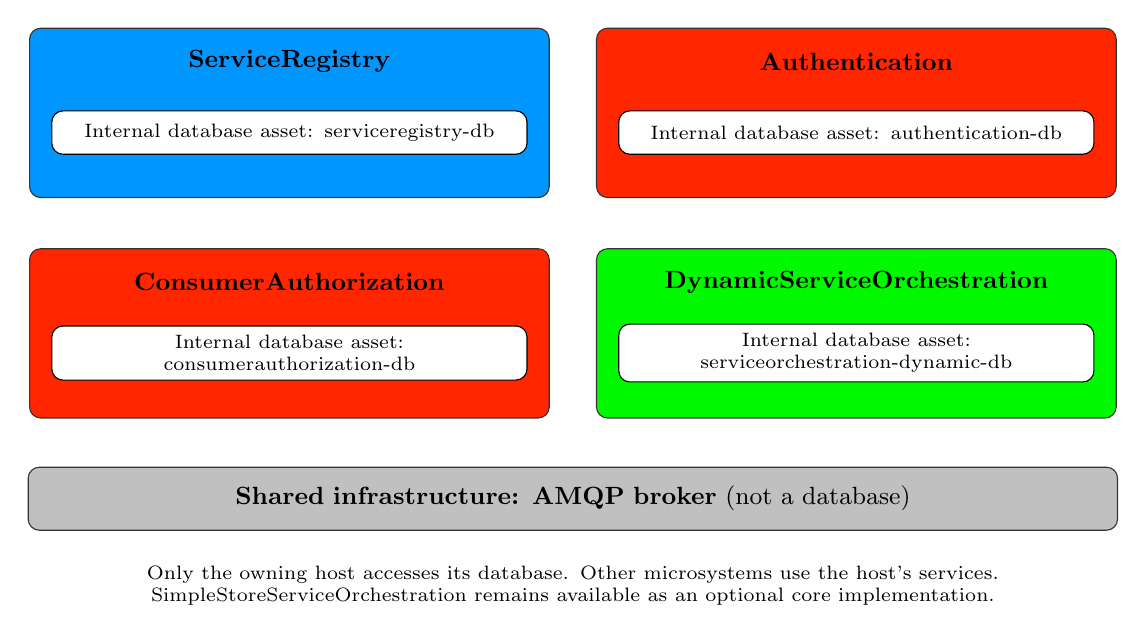
\begin{tikzpicture}[x=1cm,y=1cm,font=\small,
 host/.style={draw,rounded corners,minimum width=6.6cm,minimum height=2.15cm},
 asset/.style={draw,fill=white,rounded corners,text width=5.8cm,align=center,font=\scriptsize,minimum height=0.55cm}]
\node[host,ahRegistry] (sr) at (0,0) {};
\node at (0,0.65) {\textbf{ServiceRegistry}};
\node[asset] at (0,-0.25) {Internal database asset: serviceregistry-db};
\node[host,ahAuthentication] (auth) at (7.2,0) {};
\node at (7.2,0.65) {\textbf{Authentication}};
\node[asset] at (7.2,-0.25) {Internal database asset: authentication-db};
\node[host,ahAuthorization] (ca) at (0,-2.8) {};
\node at (0,-2.15) {\textbf{ConsumerAuthorization}};
\node[asset] at (0,-3.05) {Internal database asset: consumerauthorization-db};
\node[host,ahOrchestration] (dso) at (7.2,-2.8) {};
\node at (7.2,-2.15) {\textbf{DynamicServiceOrchestration}};
\node[asset] at (7.2,-3.05) {Internal database asset: serviceorchestration-dynamic-db};
\node[draw,rounded corners,ahInfrastructure,text width=13.6cm,align=center,minimum height=0.8cm] at (3.6,-4.9)
 {\textbf{Shared infrastructure: AMQP broker} (not a database)};
\node[text width=13.6cm,align=center,font=\scriptsize] at (3.6,-6.0)
 {Only the owning host accesses its database. Other microsystems use the host's services.\\
 SimpleStoreServiceOrchestration remains available as an optional core implementation.};
\end{tikzpicture}

\caption{New Java default design. Each database is nested inside its owning
microsystem boundary; it is not shared infrastructure or an independently
selectable component. Colors retain the established Arrowhead system roles.}
\label{fig:default-owned-assets}
\end{figure}
\FloatBarrier

\paragraph{Evidence-qualified roadmap.}
Recorded 19--24 October interoperability and federation results below remain
historical acceptance of the stated workloads. The 23 October operation-count
audit has not been replaced by a new complete differential audit. The Go
packaging audit records a failing optional native-registry integration test:
orchestration service registration is rejected, including with unmodified
reference sources. Rust still has partial DTO/error/side-effect coverage,
unsupported integrations and no automatic Java-state import. Complete
replacement requires contract, policy, persistence and mixed-cloud acceptance
for the exact image/configuration, beyond successful packaging tests
\cite{goPackaging20261028,rustPackaging20261028,nativeCompatibility20261024}.

\subsection{Support implementations and graphical engineering updates}
\label{sec:support-engineering-update}
The fifteen standalone Java support projects comprise the ten SQL-backed Spring
systems, AIGym and four native Java 21/SQLite systems. No standalone build imports
a sibling support implementation. The four native projects use JDK HttpsServer;
the retained \prop{-java-spring} folder suffix does not imply Spring. Private
common/DTO/helper source must receive fixes in each owning project. Java-cloud
LocalCloudManager remains a Node.js API with an nginx/browser UI, not a Java JAR.

Go supplies the corresponding fifteen support profiles plus LocalCloudManager,
a TestTranslation test provider and a LocalCloudConfigurator operations tool.
The 22-module packaging audit (five core and seventeen other modules) predates
the later configurator addition;
its 22-module results must not be presented as verification of all current tools.
Go LocalCloudManager is native Go with an embedded UI. Rust's fifteen support
entry points are binaries of the shared support crate, with a separate manager
crate and shared messaging. Do not describe Rust packaging as the independent
private-source closure provided by the Java and Go support distributions
\cite{javaPackaging20261025,goPackaging20261028,rustPackaging20261028}.

\paragraph{Graphical editors and authoritative state.}
LocalCloudManager's Java LC view edits a persistent, revision-guarded local-cloud
design. Databases are shown within host properties and are neither palette
components nor separate infrastructure nodes. Legacy database selections map to
the host; obsolete independent database stop flags and positions are removed by
the editor. Saving, copying, importing or repositioning a design has no runtime
effect until plan review and explicit application. The backend rejects stale
revisions and stale plan hashes \cite{javaDatabaseAssets20261030}.

The SoS view represents systems, produced/consumed service ports, connections and
nested descriptions. It persists through PDE and activates only with explicit
confirmation; diagram positions are browser presentation data. The local
orchestration editor exposes rule and security-policy editing while retaining
the provider's authentication, authorization and management checks. These views
are distinct from the SoSConfigurator operations tool, whose policy engine derives
catalogued Gatekeeper neighbours and ConsumerAuthorization grants across clouds
\cite{javaSoS20261030}.

\paragraph{Persistence is inside the microsystem boundary.}
SQL, SQLite, graph stores and private JSON snapshots are integrated host assets.
Other microsystems must use the host's produced/consumed services rather than
open its store. Ten Java Spring support databases, five core databases and the
optional GraphDBManager graph store account for the sixteen containerised assets
verified in the Java cloud. Embedded native stores remain equally private.
Host/database lifecycle ordering does not delete volumes or make scripts
transactional \cite{javaDatabaseAssets20261030}.

\paragraph{Native support release gates.}
The latest source descriptions retain limitations: Rust TimeManager reports an
untrusted host clock rather than Java SNTP trust evaluation; Onboarding's full
bootstrap/renewal/offboarding is incomplete; Choreographer and TranslationManager
have restricted workflows/adapters. Native SysMonitor and federation have dated
functional evidence, not complete Java DTO or failure-path parity. Rust manager
checks using mock sockets and its development HTTP profile do not establish secure
Java-console equivalence. Re-run exact-image security and workload acceptance
before replacing a production support system \cite{rustPackaging20261028}.



The Core systems of a local cloud provide discovery, authentication, authorisation and
orchestration \cite{gsosd50,gsosddcore}. Support systems add capabilities that many, but not all,
deployments need: richer orchestration, engineering-driven configuration of the cloud, workflow
execution, certificate life-cycle management, data and event handling, time, monitoring and
inter-cloud connectivity. The black-box \emph{GSoSD Arrowhead Support Systems 5.0}
\cite{gsosdsup50} only outlines onboarding; the remaining sections are marked ``work in
progress''. This document describes, as a white box, what exists at the 5.2 level.

\subsection{Provenance and Scope}
\label{sec:provenance}

The support systems described here have two different origins, which must not be confused:

\begin{description}
  \item[Upstream releases (Eclipse Arrowhead, v5.2.2 tags).] \sys{Blacklist}
        \cite{ah5blacklist}, \sys{TranslationManager} \cite{ah5translation} and
        \sys{DeviceQoSEvaluator} \cite{ah5qos}. Descriptions are based on the tagged
        \texttt{v5.2.2} sources.
  \item[Project migrations (EISLAB workspace).] The 13 systems of
        \prop{ah5-support-java-spring} \cite{ah5support}. They were migrated from the
        Arrowhead 4.6 core and support systems (or newly designed, as for \sys{SysMonitor} and
        \sys{AIGym}) onto the 5.2.2 Core and common library, and are deployed and tested in the
        two 5.2.2 test clouds (\prop{Arrowhead-test-cloud}, \prop{Arrowhead-test-cloud-go}).
        They are \emph{not} upstream releases. Descriptions are based on the workspace sources,
        READMEs and the per-system SysD/SysDD/SD/IDD documents.
\end{description}

Several project migrations rely on an extension of \texttt{arrowhead-common} that exists only
in the workspace: the native \svc{sysMonitor} publisher (\prop{eu.arrowhead.common.sysmonitor}).
Where a statement depends on it, this is noted.

\subsection{Document Structure}
Section~\ref{sec:prior_art} references prior art, Section~\ref{sec:use} the intended usage,
Section~\ref{sec:properties} common properties and Section~\ref{sec:delimitations} the
delimitations. Section~\ref{sec:architecture} describes the SoS architecture: system
inventory, implementation patterns, the \svc{sysMonitor} contract and the dependency graph.
Section~\ref{sec:systems} gives the white-box description of every support system.
Section~\ref{sec:services} lists produced and consumed services. Section~\ref{sec:usecases}
gives white-box use cases. Section~\ref{sec:security} covers security,
Section~\ref{sec:nfr} non-functional properties, Section~\ref{sec:ports} port allocation and
Section~\ref{sec:issues} implementation observations and open issues.

\subsection{Significant Prior Art}
\label{sec:prior_art}

\begin{itemize}
  \item \textbf{Arrowhead 4.6 (\texttt{core-java-spring}).} Choreographer, Configuration,
        DataManager, EventHandler, TimeManager, PlantDescriptionEngine, Certificate Authority,
        Onboarding controller, Gatekeeper, Gateway and QoS Monitor were 4.6 systems sharing one
        SQL database. The 5.2 migrations keep their functionality and, where sensible, their URL
        paths, but give every system its own store and adopt 5.x identities, service operations
        and naming \cite{naming2}.
  \item \textbf{GSoSD Core 5.0} \cite{gsosd50} and the white-box \textbf{Core GSoSDD 5.2.2}
        \cite{gsosddcore}: the Core services, filter chain, policies and orchestration
        approaches that all support systems build on.
  \item \textbf{External standards}: SenML (RFC 8428) \cite{rfc8428} in \sys{DataManager},
        SNTP (RFC 4330) \cite{rfc4330} in \sys{TimeManager}, PKCS\#10 (RFC 2986) \cite{rfc2986}
        and X.509 in \sys{CertificateAuthority} and \sys{Onboarding}, AMQP 0-9-1 for
        \svc{sysMonitor}, MQTT 5 for \svc{sysMonitorData} and the inter-cloud relay.
\end{itemize}

\subsection{How This SoS Is Meant to Be Used}
\label{sec:use}

Support systems are optional and deployed per need on top of a working Core local cloud. They
behave like any other microsystem: they register in the \sys{ServiceRegistry}, authenticate,
are authorised by \sys{ConsumerAuthorization}, and are found through orchestration. Six
functional groups are distinguished (Table~\ref{tab:groups}).

\begin{table}[h!]
\centering\footnotesize
\begin{tabularx}{\textwidth}{|P{3.0cm}|P{4.9cm}|Y|}\hline
\rowcolor{gray!33}Group & Systems & Purpose \\\hline
Orchestration support & \sys{Blacklist}$^U$, \sys{TranslationManager}$^U$, \sys{DeviceQoSEvaluator}$^U$ & Exclude systems, bridge incompatible interfaces/data models, rank providers by device QoS during dynamic orchestration. \\\hline
Engineering \& automation & \sys{PlantDescriptionEngine}, \sys{Choreographer}, \sys{Configuration} & Derive orchestration rules from an engineered plant description; execute workflows; distribute configuration files. \\\hline
Security \& life cycle & \sys{CertificateAuthority}, \sys{Onboarding} & Admit and withdraw devices and systems; issue and check X.509 credentials. \\\hline
Information \& messaging & \sys{EventHandler}, \sys{DataManager}, \sys{TimeManager} & Publish/subscribe events; cache and historise SenML data; trusted time. \\\hline
Monitoring \& analytics & \sys{SysMonitor}, \sys{SysMonitorPublisher} (deprecated), \sys{AIGym} & Collect and store operational telemetry of all microsystems; experiment with models on it. \\\hline
Inter-cloud & \sys{Gatekeeper}, \sys{GateTunnel} & Global service discovery, inter-cloud negotiation and tunnel/session control. \\\hline
\end{tabularx}
\caption{Functional groups of the 5.2 support systems. $^U$ = upstream v5.2.2 release; all others are EISLAB project migrations.}
\label{tab:groups}
\end{table}

\subsection{SoS Functionalities and Properties}
\label{sec:properties}

\subsubsection{Functional properties of the SoS}
\begin{itemize}
  \item \textbf{Orchestration enrichment} -- blacklisting, protocol/data-model translation
        bridges and QoS-based filtering and sorting, invoked by
        \sys{DynamicServiceOrchestration} when the corresponding \prop{enable.*} flags are set.
  \item \textbf{Engineering-driven orchestration (management layer)} --
        \sys{PlantDescriptionEngine} turns consumer/producer connections into
        managed \sys{DynamicServiceOrchestration} provider rules and raises alarms on deviations; with the
        plant-description editor of the LocalCloudManager console, its first engineering UI, it
        forms the management layer of the local cloud.
  \item \textbf{Workflow execution} -- \sys{Choreographer} runs plans of actions and steps
        (a DAG per action) on registered executors, with orchestration made for each executor.
  \item \textbf{Admission control and credential life cycle} -- \sys{Onboarding} admits
        operator-approved devices and their systems step by step (onboarding, device and system
        certificates, identities) and off-boards them again; \sys{CertificateAuthority} signs,
        checks and revokes end-entity certificates and manages trusted keys.
  \item \textbf{Data, events, time, configuration} -- SenML proxy and historian, event
        publish/subscribe with metadata filtering, NTP-checked trusted time, per-system
        configuration files.
  \item \textbf{Monitoring} -- every microsystem publishes \svc{sysMonitor} observations
        (\op{echo}, \op{power}, \op{status}) over AMQPS; \sys{SysMonitor} discovers, subscribes,
        stores and republishes them over MQTT; \sys{PlantDescriptionEngine} and \sys{AIGym} use
        them.
  \item \textbf{Inter-cloud exchange} -- Gatekeeper global service discovery and inter-cloud
        negotiation, and GateTunnel sessions, carried between local clouds by an
        organisation-level MQTT relay with a name-constrained organisation PKI.
\end{itemize}

\subsubsection{Configuration of SoS properties}
Spring systems are configured through \prop{application.properties}; the Java 21
independently packaged native Java systems (\sys{CertificateAuthority}, \sys{Gatekeeper},
\sys{GateTunnel}, \sys{SysMonitor}) use environment variables. Their former Python
backends were replaced on 16 October 2026. Common switches are those of the Core (\prop{authentication.policy},
\prop{server.ssl.*}, \prop{management.policy}, \prop{enable.blacklist.filter}) plus:
\begin{itemize}
  \item \prop{service.authorization.enabled} (\sys{TimeManager}, \sys{DataManager},
        \sys{Configuration}, \sys{PlantDescriptionEngine}): per-call
        \svc{authorization}~\op{verify} of produced application services, cached 30\,s and
        failing closed. The secure default profile enables this enforcement. A
        component sample that sets it to \texttt{false} is a development exception;
        registration or orchestration alone does not authorise a provider call.
  \item \prop{sysmonitor.enabled}, \prop{sysmonitor.broker.*}, \prop{sysmonitor.ssl.*},
        \prop{sysmonitor.local.cloud}, \prop{sysmonitor.publish.interval} (default 30\,s): the
        native \svc{sysMonitor} publisher.
\end{itemize}

\subsubsection{Data stored by the individual microsystems}
Every support system owns its data (Table~\ref{tab:inventory}); none shares a schema with
another system. Spring systems use their own MySQL schema, accessed with MariaDB
Connector/J (\texttt{jdbc:mariadb}, TLS with full verification). The four
independent native Java systems retain private SQLite stores. \sys{AIGym} and \sys{SysMonitorPublisher} keep only volatile state.

\subsubsection{Non-functional properties}
\begin{itemize}
  \item \textbf{Security}: full AA and encrypted information exchange are the default
        from v5.0. The Java reference realises this through mutual TLS, \texttt{OUTSOURCED}
        authentication with identity tokens bound to the certificate CN, \texttt{CERT\_AUTH}
        interface policy, ConsumerAuthorization grants per service, and
        \texttt{sysop-only} management. The independent native Java systems have no insecure mode.
  \item \textbf{Observability}: uniform liveness, power and status telemetry with
        \texttt{alive}/\texttt{degraded} semantics tied to each system's own health (database,
        NTP trust, synchronisation alarms).
  \item \textbf{Robustness}: failure of a support system never stops the Core; orchestration
        features degrade to warnings or, where forced, fail closed.
  \item \textbf{Scalability}: all systems are designed for one active instance; replication
        needs shared stores (explicitly stated for \sys{CertificateAuthority} and
        \sys{SysMonitor}).
\end{itemize}

\subsubsection{Stateful or stateless}
All systems except \sys{AIGym} (ephemeral models) and \sys{SysMonitorPublisher} are stateful.
Long-lived state: blacklist entries, translation bridges, device statistics, plant descriptions
and alarms, plans and sessions, configuration files, issued certificates and trusted keys,
event subscriptions, SenML history, observation history, cloud/relay records and tunnel
sessions. \sys{TimeManager} keeps only logs.

\subsection{Important Delimitations}
\label{sec:delimitations}

\begin{itemize}
  \item Upstream systems are described at their \texttt{v5.2.2} tags; workspace modifications
        of those repositories (removal of the \svc{monitor} service, native \svc{sysMonitor})
        are noted but are not part of the release.
  \item Project migrations retain their original 13 October descriptions, with dated
        implementation and packaging updates through 30 October. They are
        not released, not reviewed by the Eclipse Arrowhead project, and may change.
  \item Inter-cloud exchange is provided by the project implementations of \sys{Gatekeeper} and
        \sys{GateTunnel} over the inter-cloud relay (Section~\ref{sec:relay}), between local clouds
        of the same organisation. The upstream 5.2.2 release has no counterpart for
        \sys{DynamicServiceOrchestration}'s \prop{enable.intercloud}.
  \item Human identity federation, automated OCSP, ACME/EST/SCEP and automatic CA
        key rotation are not provided. CRL publication and configured enforcement
        are implemented; operator console password sessions are a separate mechanism.
  \item \sys{LocalCloudManager}, the operator tool of the test clouds, is a client of these
        systems and is not described.
\end{itemize}

\newpage
%% ============================================================================================
\section{SoS Architecture}
\label{sec:architecture}

\subsection{System Inventory}

{\footnotesize
\begin{longtable}{|P{3.3cm}|P{0.9cm}|P{2.3cm}|P{3.5cm}|P{5.3cm}|}\hline
\rowcolor{gray!33}Microsystem & Port & Technology & Persistence & Origin \\\hline\endhead
\sys{Blacklist}$^U$ & 8464 & Java 21, Spring Boot & MySQL \texttt{ah\_blacklist} & New in 5.x \\\hline
\sys{TranslationManager}$^U$ & 8465 & Java 21, Spring Boot & MySQL \prop{ah_translation_manager} & New in 5.x (successor of the 4.x Translator) \\\hline
\sys{DeviceQoSEvaluator}$^U$ & 8472 & Java 21, Spring Boot, Quartz; Python device agent & MySQL \prop{ah_device_qos_evaluator} & New in 5.x (successor of 4.6 QoS Monitor) \\\hline
\sys{PlantDescriptionEngine} & 8432 & Java 21, Spring Boot & MariaDB \prop{ah_plantdescriptionengine} & 4.6 PlantDescriptionEngine \\\hline
\sys{Choreographer} & 8457 & Java 21, Spring Boot & MariaDB \texttt{ah\_choreographer} & 4.6 Choreographer (core) \\\hline
\sys{Configuration} & 8459 & Java 21, Spring Boot & MariaDB \texttt{ah\_configuration} & 4.6 Configuration (core) \\\hline
\sys{CertificateAuthority} & 8448 & Java 21, own JAR & SQLite & 4.6 Certificate Authority \\\hline
\sys{Onboarding} & 8435 & Java 21, Spring Boot 3.4.9 & MariaDB \texttt{ah\_onboarding} (enrolments, logs) & 4.6.2 Onboarding controller; procedure of \cite{bicaku2018} \\\hline
\sys{EventHandler} & 8455 & Java 21, Spring Boot & MariaDB \texttt{ah\_eventhandler} & 4.6 EventHandler (core) \\\hline
\sys{DataManager} & 8461 & Java 21, Spring Boot & MariaDB \texttt{ah\_datamanager} & 4.6 DataManager \\\hline
\sys{TimeManager} & 8463 & Java 21, Spring Boot & MariaDB \texttt{ah\_timemanager} (logs) & 4.6 TimeManager (core) \\\hline
\sys{SysMonitor} & 8475 & Java 21, AMQP intake, MQTT output & SQLite & New (5.0 draft SysD ``MicrosystemMonitor'') \\\hline
\sys{SysMonitorPublisher} & -- & container sidecar & none & New; deprecated 2026-10-11 \\\hline
\sys{AIGym} & 8478 & Java & in memory & 4.6 \prop{rsafg-ai-gym-client} \\\hline
\sys{Gatekeeper} & 8449 & Java 21, own JAR & SQLite & 4.6 Gatekeeper \\\hline
\sys{GateTunnel} & 8453 & Java 21, own JAR & SQLite & 4.6 Gateway \\\hline
\caption{Inventory of the 5.2 support systems (canonical ports, Section~\ref{sec:ports}). $^U$ = upstream v5.2.2 release.}
\label{tab:inventory}
\end{longtable}
}

\subsection{Implementation Patterns}

\paragraph{Spring systems on \texttt{arrowhead-common}.} The Spring systems share the internal
architecture described for the Core in \cite{gsosddcore}: \texttt{SystemInfo} declaring system
and service models, \prop{ApplicationInitListener} performing SR registration,
the ordered filter chain (authentication $\rightarrow$ blacklist $\rightarrow$ management),
validation and normalisation, a service layer, engines/drivers, JPA persistence in a private
schema, Quartz or scheduled cleaner jobs, and \svc{generalManagement}
(\op{get-log}, \op{get-config}). The workspace common library now advertises
\texttt{CERT\_AUTH} for HTTPS interfaces by default (23 October 2026); some services
retain explicit registration overrides. This is distinct from the released
library's older \texttt{NONE} behaviour.

\paragraph{Independently packaged native Java systems.} \sys{CertificateAuthority}, \sys{Gatekeeper},
\sys{GateTunnel} and \sys{SysMonitor} run natively in Java 21, with mandatory mutual
TLS, certificate-bound identities, service-specific authorisation and SQLite
persistence. They bootstrap through ServiceRegistry and use orchestration for
ordinary service consumption. The 25 October packaging provides a fixed Java entry point, own Maven build, image, environment template and Compose definition in each system folder. Helpers are private source copies and SQLite volumes are system-owned; separate health checks remain infrastructure. The live-cloud baseline remains the previously deployed image until the operator rolls out the new packaging.
The Python RandomDataProducer is an application, not one of these support backends
\cite{javaDeployment20261024}.


\subsection{Independent native Java support deployments}
\label{sec:independent-support}
CertificateAuthority, Gatekeeper, GateTunnel and SysMonitor are independently buildable and deployable from their respective folders in the Eclipse-Arrowhead distribution. Each folder owns its source, Maven POM, tests, fixed main class, shaded JAR, Dockerfile, environment template and Compose definition. No build context or source import points to a sibling support system. No common support runtime image, runtime role selector, shared database or common configuration bundle is required.

\begin{figure}[htbp]
\centering
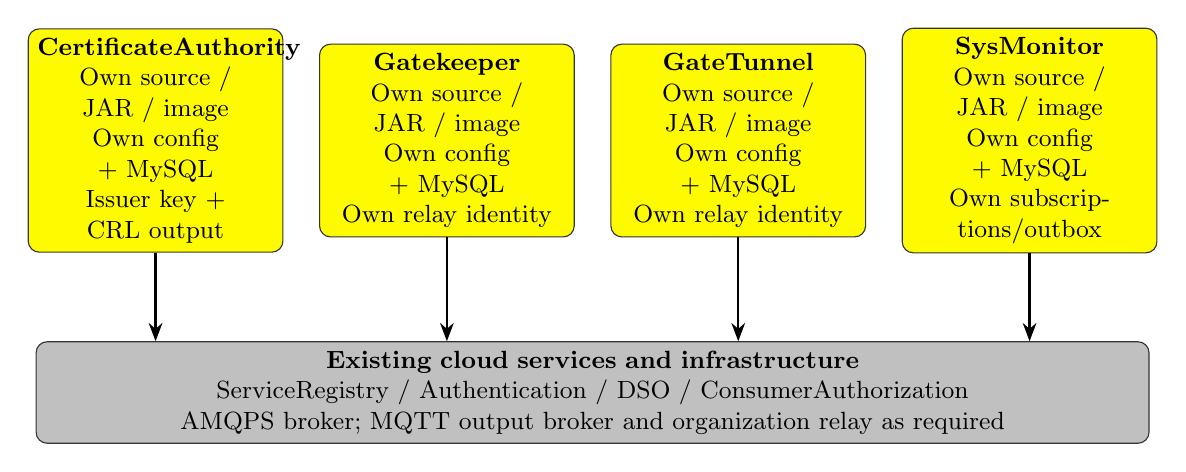
\begin{tikzpicture}[b/.style={draw,rounded corners,align=center,text width=3.0cm,minimum height=2.0cm,font=\small}, >=Stealth]
\node[b,ahSupport] (ca) at (0,0) {\textbf{CertificateAuthority}\\Own source / JAR / image\\Own config + MySQL\\Issuer key + CRL output};
\node[b,ahSupport] (gk) at (3.7,0) {\textbf{Gatekeeper}\\Own source / JAR / image\\Own config + MySQL\\Own relay identity};
\node[b,ahSupport] (gt) at (7.4,0) {\textbf{GateTunnel}\\Own source / JAR / image\\Own config + MySQL\\Own relay identity};
\node[b,ahSupport] (sm) at (11.1,0) {\textbf{SysMonitor}\\Own source / JAR / image\\Own config + MySQL\\Own subscriptions/outbox};
\node[draw,ahInfrastructure,rounded corners,align=center,text width=13.9cm,minimum height=1.2cm,font=\small] (services) at (5.55,-3.2) {\textbf{Existing cloud services and infrastructure}\\ServiceRegistry / Authentication / DSO / ConsumerAuthorization\\AMQPS broker; MQTT output broker and organization relay as required};
\foreach \n in {ca,gk,gt,sm} {\draw[->,thick] (\n.south) -- (\n.south |- services.north);}
\end{tikzpicture}

\caption{Independent support packaging and private state. Arrows denote network service use, not shared implementation or data. Operators select the support systems needed by their local cloud.}
\label{fig:independent-support}
\end{figure}

The four project folders are \prop{ah5-CertificateAuthority-java-spring}, \prop{ah5-Gatekeeper-java-spring}, \prop{ah5-GateTunnel-java-spring} and \prop{ah5-SysMonitor-java-spring}. Their implementations use Java 21 and JDK HttpsServer; the retained folder naming does not imply a Spring dependency. The artifact names are respectively \prop{arrowhead-certificate-authority}, \prop{arrowhead-gatekeeper}, \prop{arrowhead-gatetunnel} and \prop{arrowhead-sysmonitor}, version 5.2.2.

Build and verify within a selected folder using \prop{mvn -B clean verify}, or build its local Dockerfile. Deployment uses that folder's \prop{compose.yaml} and \prop{.env.example}; the operator provisions its own system identity, password file, trusted CA, CRL and selected external network. Each Compose project owns its private SQLite volume. Containers run as UID 10001 with a read-only root filesystem and bounded non-executable temporary storage. The platform SQLite native library is installed in the image at build time rather than extracted into temporary storage at runtime. Only CertificateAuthority mounts the issuer signing key and writes the published CRL. Other systems receive public trust material, their own identity and a read-only CRL. CRL distribution is an explicit cloud operation.

Independence concerns packaging and state ownership. ServiceRegistry remains the bootstrap service; Authentication and DynamicServiceOrchestration are discovered there, and ordinary consumption follows DSO and authorization rules. AMQPS monitoring, SysMonitor's MQTT output and federation's organization MQTT relay remain network dependencies. Gatekeeper and GateTunnel cooperate for inter-cloud service use, without forcing a combined artifact or process. AH-GT-1 is supported and selected in the federation Compose samples; compatibility with legacy-mTLS is explicit and does not permit silent downgrade.

Common helpers are copied privately into each project. Security changes to these copies must be propagated and tested in every affected project. Historical implementations remain under each project's \prop{legacy/}; the copied combined runtime is reference material and is not used by the independent projects. The remaining Spring projects are independently packaged as specified in the following complete-distribution section; third-party Maven libraries remain normal dependencies.

The per-system SysDDs specify these build and deployment boundaries. Verification uses isolated builds, generated test identities, role startup, security and contract tests, shaded-JAR inspection, SQLite smoke checks and image/configuration checks. The distribution's verification report records the results. This document describes deployable packaging and does not assert a new live-cloud deployment.

\subsection{Complete selectable Java support distribution}
The standalone distribution now covers all fifteen Java support systems, not only the four former native runtime roles. Each project owns its application source, executable JAR, Dockerfile, configuration, tests and Compose definition. The standalone support project builds do not read JavaSupportRuntime or a sibling support project. Existing cloud deployment consumers may retain historical build contexts until deliberately retargeted.

The ten database-backed Spring systems (Blacklist, TranslationManager, DeviceQoSEvaluator, Onboarding, DataManager, TimeManager, EventHandler, PlantDescriptionEngine, Configuration and Choreographer) compile private Arrowhead common utilities and DTO source under \prop{vendor/}. Their POMs inherit only the published Spring Boot parent; no Arrowhead common/core parent or preinstalled Arrowhead library is required. Local provenance manifests preserve source hashes, licensing and upstream POMs. Source security fixes must be propagated to every affected private copy. AIGym keeps its existing independent Spring Boot build. The four native Java systems retain their separate helpers and shaded JARs.

Each database-backed deployment starts its own MySQL instance and initializes only its own schema on a fresh project volume. The DB has no host port, has an operator-selected private subnet and requires TLS. Application and database passwords are independent file secrets. App credentials and trust are mounted individually; the app sees the public database CA but no DB key or CA signing key. The production configuration requires mutual TLS, outsourced authentication, certificate/token binding and a valid CRL. Containers use an unprivileged application user and a read-only root filesystem. Database credentials and schemas are not shared across selected support systems.

Packaging independence preserves network contracts. ServiceRegistry, Authentication, DSO, ConsumerAuthorization and required brokers/providers must be provisioned in the selected cloud. Some systems refuse startup until core services are available. Deployment tests therefore use isolated mutual-TLS registry/authentication/DSO protocol fixtures, own test credentials and private databases, with one support system selected at a time. Authorized HTTPS requests and missing-token/certificate rejection are checked. Listener checks alone do not establish application, monitoring, federation or NTP readiness; the distribution verification report states exact coverage and limitations.

LocalCloudManager is an explicit non-Java exception: its existing implementation is Node.js/nginx. It owns API/UI sources, npm tests, images and an independent console Compose definition; a Java JAR is not applicable. The console-only deployment has no Docker host-control service. The copied core project and historical combined runtime are not support-system deployment units in this inventory.

The distribution \prop{DEPLOYMENT-GUIDE.md}, each project \prop{DEPLOYMENT.md} and the all-system verification report specify project names, host ports, private subnets, credential provisioning, build commands and state lifecycle. The per-system SysDDs describe the new packaging. Existing live-cloud evidence remains historical baseline; this packaging change does not redeploy live clouds.

\subsection{The sysMonitor Contract}
\label{sec:sysmonitor}

Monitoring is the cross-cutting concern that ties the support systems together
(Figure~\ref{fig:monitoring}).

\begin{itemize}
  \item Every microsystem produces a \svc{sysMonitor} 1.0.0 service with interface
        \texttt{generic\_amqps}, policy \texttt{CERT\_AUTH} and metadata
        \prop{publisherMode=native}; the \texttt{generic\_amqp}/\texttt{generic\_amqps} interface
        templates are created in the \sys{ServiceRegistry} at deployment.
  \item Each operation is the periodic publication (default every 30\,s) of one observation type
        to the AMQP topic exchange \texttt{arrowhead} of the cloud's AMQP broker (RabbitMQ 4.0,
        AMQP 0-9-1 over TLS, port 5671) with routing key
        \prop{<cloud>.sysmonitor.<System>.<serviceInstance>.<type>}; baseline types are \op{echo}
        (\texttt{alive} or \texttt{degraded}), \op{power} and \op{status}. Messages are persistent and
        confirmed by the broker.
  \item Publishers authenticate with their own certificate (SASL \texttt{EXTERNAL}: the broker user
        is the certificate CN). The broker's access list names, per CN, the routing keys a system
        may publish and the binding keys it may bind its own queues with; every system may publish
        only below its own routing key, and \sys{SysMonitor} may bind
        \prop{<cloud>.sysmonitor.*.*.*}.
  \item The observation envelope carries \texttt{schemaVersion}, \texttt{observationId},
        \texttt{providerSystem}, \texttt{serviceInstance}, \texttt{observationType},
        \texttt{sourceTime}, a monotonic \texttt{sequence}, \texttt{value}, \texttt{unit},
        \texttt{quality} and \texttt{metadata} \cite{sysmonidd}.
  \item \sys{SysMonitor} needs a ConsumerAuthorization grant \prop{<System>|sysMonitor} for every
        provider. Publishers are the common-library \texttt{SysMonitorPublisher} (Java systems),
        the RabbitMQ Java client (native Java and \sys{AIGym}), the Java
        \sys{ServiceRegistry}, pika (RandomDataProducer) and amqplib (LocalCloudManager).
  \item The AMQP broker carries only \svc{sysMonitor}. The MQTT broker (Mosquitto 2.0, port 8883)
        stays in place for \svc{sysMonitorData} and all other intra-cloud MQTT traffic.
  \item HTTPS liveness probes, where still present, are registered as service \svc{echo}
        (never as \svc{monitor}, \svc{monitoring} or \svc{sysMonitor}).
\end{itemize}

\begin{figure}[h!]
\centering
\begin{tikzpicture}[scale=0.9, every node/.style={transform shape}]
  \node[appbox, minimum width=3.4cm, ahMixed] (any) at (-7.2,0) {Any microsystem\\(Core, Support, App)};
  \node[draw=ArrowheadGrey, thick, fill=AHSysMLInfrastructure, minimum width=2.8cm, minimum height=1cm, align=center, ahInfrastructure] (broker) at (-1.8,0) {AMQP broker\\{\scriptsize RabbitMQ, mTLS + ACL}};
  \node[supbox, minimum width=3.2cm, ahSupport] (sm) at (3,0) {SysMonitor\\{\scriptsize SQLite history}};
  \node[sysbox, minimum width=3.4cm, ahOrchestration] (dso) at (3,2.4) {DynamicService-\\Orchestration};
  \node[sysbox, minimum width=3.4cm, ahAuthorization] (ca) at (-3.4,2.4) {ConsumerAuthorization};
  \node[supbox, ahSupport] (pde) at (7.4,1.2) {PlantDescription-\\Engine};
  \node[draw=ArrowheadGrey, thick, fill=AHSysMLInfrastructure, minimum width=2.8cm, minimum height=1cm, align=center, ahInfrastructure] (mqtt) at (3,-2.4) {MQTT broker\\{\scriptsize Mosquitto, mTLS + ACL}};
  \node[supbox, ahSupport] (ai) at (-1.8,-2.4) {AIGym};
  \node[appbox, ahApplication] (an) at (7.4,-2.4) {Analytics consumers};
  \draw[msg] (any) -- node[lbl, above]{\svc{sysMonitor}} (broker);
  \draw[msg] (broker) -- node[lbl, above]{queue} (sm);
  \draw[msg] (sm) -- node[lbl, right]{\op{pull} \svc{sysMonitor}} (dso);
  \draw[msg] (dso) -- node[lbl, above]{\op{check-policies}} (ca);
  \draw[msg] (pde) -- node[lbl, above, pos=0.4]{history} (sm);
  \draw[msg] (sm) -- node[lbl, right]{\svc{sysMonitorData}} (mqtt);
  \draw[msg] (mqtt) -- (ai);
  \draw[msg] (mqtt) -- (an);
\end{tikzpicture}
\caption{Monitoring chain: observations over AMQP into SysMonitor, history over HTTPS, normalised
stream over MQTT.}
\label{fig:monitoring}
\end{figure}

\subsection{Dependency Graph}

Figure~\ref{fig:deps} shows which Core and Support services each support system consumes.
PDE, Choreographer, SysMonitor and AIGym use DynamicServiceOrchestration. SimpleStore
remains an independent optional system; it is no longer a dependency of PDE. The local
managed-plant API and schema upgrade are described in Section~\ref{sec:pde-dso}.

\begin{figure}[h!]
\centering
\begin{tikzpicture}[scale=0.82, every node/.style={transform shape}]
  % core row
  \node[sysbox, minimum width=2.9cm, ahRegistry] (sr)  at (0,0)   {ServiceRegistry};
  \node[sysbox, minimum width=2.9cm, ahAuthentication] (au)  at (-6.4,0) {Authentication};
  \node[sysbox, minimum width=2.9cm, ahAuthorization] (ca)  at (-3.2,0) {Consumer-\\Authorization};
  \node[sysbox, minimum width=2.9cm, ahOrchestration] (dso) at (3.2,0) {DynamicService-\\Orchestration};
  \node[sysbox, minimum width=2.9cm, ahOrchestration] (sso) at (6.4,0) {SimpleStoreService-\\Orchestration};
  % support above
  \node[supbox, minimum width=2.6cm] (bl)  at (0.6,3.0)  {Blacklist};
  \node[supbox, minimum width=2.6cm, ahSupport] (tm)  at (3.6,3.0)  {Translation-\\Manager};
  \node[supbox, minimum width=2.6cm, ahSupport] (qos) at (6.6,3.0)  {DeviceQoS-\\Evaluator};
  \node[supbox, minimum width=2.6cm, ahSupport] (gk)  at (-2.4,3.0) {Gatekeeper};
  \node[supbox, minimum width=2.6cm, ahSupport] (gt)  at (-5.4,3.0) {GateTunnel};
  % support below
  \node[supbox, minimum width=2.4cm, ahSupport] (pde) at (6.4,-3.0) {PlantDescr.-\\Engine};
  \node[supbox, minimum width=2.4cm, ahSupport] (ch)  at (3.6,-3.0) {Choreographer};
  \node[supbox, minimum width=2.4cm, ahSupport] (sm)  at (0.8,-3.0) {SysMonitor};
  \node[supbox, minimum width=2.4cm, ahSupport] (ai)  at (0.8,-5.0) {AIGym};
  \node[supbox, minimum width=2.4cm, ahSupport] (ob)  at (-2.0,-3.0) {Onboarding};
  \node[supbox, minimum width=2.4cm, ahSupport] (cert) at (-2.0,-5.0) {Certificate-\\Authority};
  \node[supbox, minimum width=2.4cm, ahSupport] (oth) at (-5.6,-3.0) {TimeManager, DataMgr,\\Configuration,\\EventHandler};

  \draw[opt] (dso) -- (bl); \draw[opt] (dso) -- (tm); \draw[opt] (dso) -- (qos);
  \draw[uses] (tm) -- (ca); \draw[uses] (tm.south west) -- (sr);
  \draw[uses] (qos) -- (sr);
  \draw[uses] (gk) -- (sr); \draw[uses] (gt) -- (au);
  \draw[uses] (pde) -- (dso); \draw[uses] (pde) -- (sr); \draw[uses] (pde) -- (sm);
  \draw[uses] (ch) -- (dso); \draw[uses] (sm) -- (dso); \draw[uses] (ai) -- (sm); \draw[uses] (ai.north east) -- (dso);
  \draw[uses] (ob) -- (sr); \draw[uses] (ob) -- (cert);
  \draw[uses] (oth) -- (ca); \draw[uses] (oth) -- (au);
\end{tikzpicture}
\caption{Consumption dependencies of the support systems (dashed: invoked by
\texttt{DynamicServiceOrchestration} when enabled). Registration in the ServiceRegistry and
identity/authorisation calls of every system are omitted for clarity.}
\label{fig:deps}
\end{figure}

\newpage
%% ============================================================================================

\FloatBarrier
\subsection{Deployed Java Reference Cloud (24 October 2026)}
\label{sec:java-deployment}
The local Java reference deployment is the Docker Compose project
\prop{arrowhead-v52-test-cloud}, maintained in \prop{Arrowhead-test-cloud-java}.
Figure~\ref{fig:java-deployment} records its 22 deployed microsystems, including
both orchestration variants, the operations manager and the demonstration application
\cite{javaDeployment20261024}. This is a dated deployment example of the architecture,
not a requirement that every local cloud deploy every optional support system.
In this 24 October snapshot, the five Core systems and fifteen support systems
are Java implementations;
\sys{LocalCloudManager} has a Node.js API and \sys{RandomDataProducer} is a Python
application. Thus ``Java cloud'' identifies the reference implementation baseline,
not the language of every process.

\begin{figure}[htbp]
\centering
% Deployment snapshot, 24 October 2026. Editable vector artwork.
\begin{tikzpicture}[x=1cm,y=1cm,
  block/.style={draw=ArrowheadBlue,fill=ArrowheadBlue!4,rounded corners=2pt,
  text width=3.55cm,align=center,font=\scriptsize,inner sep=4pt},
  route/.style={-{Stealth[length=2mm]},thick,ArrowheadBlue}]
\node[block,text width=15.3cm,minimum height=0.9cm, ahMixed] (bus) at (6,0)
 {\textbf{Common service-consumption contract}\\
 ServiceRegistry discovery $\rightarrow$ Authentication identity $\rightarrow$
 service orchestration $\rightarrow$ direct, authorised provider call};
\node[block,anchor=north,minimum height=5.4cm, ahMixed] (core) at (0,-1.1)
 {\textbf{Core (5; private owned state)}\\[5pt]
 \colorbox{AHSysMLRegistry}{\parbox{3.1cm}{\centering ServiceRegistry}}\\[4pt]
 \colorbox{AHSysMLSecurity}{\parbox{3.1cm}{\centering Authentication}}\\[4pt]
 \colorbox{AHSysMLSecurity}{\parbox{3.1cm}{\centering ConsumerAuthorization}}\\[4pt]
 \colorbox{AHSysMLOrchestration}{\parbox{3.1cm}{\centering DynamicService-\\Orchestration}}\\[4pt]
 \colorbox{AHSysMLOrchestration}{\parbox{3.1cm}{\centering SimpleStoreService-\\Orchestration}}};
\node[block,anchor=north,minimum height=5.4cm, ahSupport] (life) at (4,-1.1)
 {\textbf{Lifecycle and policy (4)}\\[5pt]
 Blacklist\\[7pt] Onboarding\\[7pt] CertificateAuthority\\[7pt] DeviceQoSEvaluator};
\node[block,anchor=north,minimum height=5.4cm, ahSupport] (svc) at (8,-1.1)
 {\textbf{Data and engineering (7)}\\[5pt]
 TranslationManager\\[4pt] DataManager\\[4pt] TimeManager\\[4pt] EventHandler\\[4pt]
 Configuration\\[4pt] PlantDescriptionEngine\\[4pt] Choreographer};
\node[block,anchor=north,minimum height=5.4cm, ahMixed] (ops) at (12,-1.1)
 {\textbf{Operations and exchange (6)}\\[5pt]
 \colorbox{AHSysMLSupport}{\strut SysMonitor}\\[4pt] \colorbox{AHSysMLSupport}{\strut AIGym}\\[4pt] \colorbox{AHSysMLSupport}{\strut Gatekeeper}\\[4pt] \colorbox{AHSysMLSupport}{\strut GateTunnel}\\[4pt]
 \colorbox{AHSysMLSupport}{\strut LocalCloudManager}\\[4pt]\colorbox{AHSysMLApplication}{\strut RandomDataProducer}};
\foreach \n in {core,life,svc,ops} \draw[route] (bus.south -| \n.north) -- (\n.north);
\node[block,text width=15.3cm,minimum height=1cm, ahMixed] (monitor) at (6,-7.5)
 {\textbf{Native monitoring from all 22 microsystems}\\
 AMQP broker $\rightarrow$ SysMonitor (SQLite history/outbox)
 $\rightarrow$ MQTT broker $\rightarrow$ AIGym};
\draw[route] (ops.south) -- (ops.south |- monitor.north);
\node[block,text width=15.3cm,fill=gray!6,draw=ArrowheadGrey, ahInfrastructure] at (6,-9)
 {\textbf{Integrated assets:} 15 private MySQL containers owned by their microsystems.\\
 \textbf{Infrastructure:} AMQP and MQTT brokers; dashboard UI; constrained Docker proxy.\\
 24 October snapshot: 41 containers. The federation relay is a separate project.};
\end{tikzpicture}

\caption{Deployed Java reference cloud. All 22 named systems are microsystems;
message brokers, dashboard and Docker proxy are infrastructure; database
containers are integrated assets inside their host microsystems.
The shared consumption path is drawn once to avoid repeating bootstrap edges.}
\label{fig:java-deployment}
\end{figure}
\FloatBarrier

The 41 running containers comprise the 22 microsystems, 15 dedicated MySQL
containers, two message brokers, a dashboard UI and a Docker proxy. The four
\sys{CertificateAuthority}, \sys{Gatekeeper}, \sys{GateTunnel} and \sys{SysMonitor}
services use independently packaged Java 21 implementations, each retaining its own SQLite state.
The former delegated \sys{SysMonitorPublisher} is not a deployed microsystem:
each system publishes its own \svc{sysMonitor} observations.

\paragraph{Discovery, orchestration and direct consumption.}
Systems bootstrap through \sys{ServiceRegistry}, locate \svc{identity} and
\svc{serviceOrchestration}, obtain a certificate-bound identity token and request
an authorised provider for the required operation. The resulting call goes from
consumer to provider; the orchestrator does not proxy the application payload.
DSO directly discovers its own authorisation and blacklist dependencies to avoid
recursive orchestration. Authentication also bootstraps its authorisation check.
Other dependency calls use orchestration, with the documented caches and exceptions.

\paragraph{Monitoring and application data.}
Native publishers send observations over AMQPS to RabbitMQ; \sys{SysMonitor}
consumes authorised selections and stores them in its own SQLite history/outbox.
It republishes normalised \svc{sysMonitorData} through MQTT for \sys{AIGym}.
\sys{LocalCloudManager} reads \svc{sysMonitorHistory} and manages subscriptions.
The demonstration producer instead writes application SenML data to
\sys{DataManager} every 30\,s through \svc{dataHistorian}~\op{put-data}.
Monitoring history is not stored by DataManager.

\paragraph{Engineering, workflow and federation paths.}
The plant editor calls \sys{PlantDescriptionEngine}; an active plant is compiled
into an atomic DSO rule snapshot through \svc{serviceOrchestrationPlantManagement}.
\sys{Choreographer} asks DSO for push orchestration on behalf of workflow executors;
no executor is deployed by default. Onboarding consumes certificate signing,
validation and revocation, identity management and blacklist operations.
Inter-cloud selection uses Gatekeeper discovery/negotiation and an AH-GT-1
GateTunnel session over the external relay. The 24 October deployment snapshot contained
neither SimpleStore route rows nor an active DSO plant-rule row: these mechanisms
are available, but the diagram does not imply an active engineered workflow.

\paragraph{Reference security profile.}
The deployed service profile realises the v5.0-and-later default: full AA and
information encryption, using mutual TLS with \texttt{CERT\_AUTH}, certificate-bound
identity tokens and operation-scoped authorisation. Unsecured component samples
are explicit development exceptions, not an alternative architectural default. The operator console requires login and reaches
Docker only through a project-scoped proxy. CertificateAuthority publishes CRLs;
services and brokers enforce them on new TLS handshakes. Ending established
connections is a separate action. AH-GT-1 protects relayed payloads end to end;
cloud application trust remains separate from relay/organisation trust
\cite{javaDeployment20261024,rustFederation20261019}.

\subsection{Support-System Paths in the Deployed Cloud}
\begin{figure}[htbp]
\centering
% Main service paths; arrows show service/data direction, not a traffic trace.
\begin{tikzpicture}[x=1cm,y=1cm,
 b/.style={draw=ArrowheadBlue,fill=ArrowheadBlue!4,rounded corners=2pt,
 text width=4.2cm,align=center,font=\scriptsize,minimum height=0.95cm},
 a/.style={-{Stealth[length=2mm]},thick,ArrowheadBlue},
 t/.style={font=\scriptsize,fill=white,align=center,text width=3.8cm,inner sep=2pt}]
\node[b, ahApplication] (rdp) at (0,0) {RandomDataProducer};
\node[b, ahOrchestration] (dso) at (5.3,0) {DynamicServiceOrchestration};
\node[b, ahSupport] (dm) at (10.6,0) {DataManager\\dataHistorian / dataProxy};
\draw[a] (rdp) -- node[t,below=18pt]{service requirement} (dso);
\draw[a,dashed] (dso) -- node[t,above=18pt]{discovers / selects provider} (dm);
\draw[a] (dso.north west) to[bend right=40] node[t,above=2pt]{returns endpoint to consumer} (rdp.north east);
\draw[a] (rdp.south) -- ++(0,-1.25) -| (dm.south);
\node[t,text width=10cm] at (5.3,-1.95) {consumer calls provider: put-data every 30 s};
\node[b, ahSupport] (ui) at (0,-3.2) {LocalCloudManager\\plant editor};
\node[b, ahSupport] (pde) at (5.3,-3.2) {PlantDescriptionEngine};
\node[b, ahOrchestration] (plant) at (10.6,-3.2) {DSO managed plant snapshot};
\draw[a] (ui) -- node[t,above=18pt]{plant descriptions} (pde);
\draw[a] (pde) -- node[t,above=18pt]{query / replace} (plant);
\node[b, ahSupport] (ch) at (0,-5.5) {Choreographer};
\node[b, ahOrchestration] (push) at (5.3,-5.5) {DSO push orchestration};
\node[b, ahApplication] (ex) at (10.6,-5.5) {Executor step\\not deployed by default};
\draw[a] (ch) -- node[t,below=18pt]{executor's service requirement} (push);
\draw[a] (push.north west) to[bend right=40] node[t,above=2pt]{result callback} (ch.north east);
\draw[a,dashed] (ch.south) -- ++(0,-1.25) -| (ex.south);
\node[t,text width=10cm] at (5.3,-7.2) {Choreographer starts executor with the result};
\node[b, ahMixed] (gk) at (0,-9) {\colorbox{AHSysMLOrchestration}{\strut DSO / SimpleStore}\\$\rightarrow$ \colorbox{AHSysMLSupport}{\strut Gatekeeper}};
\node[b, ahSupport] (gt) at (5.3,-9) {GateTunnel};
\node[b, ahInfrastructure] (peer) at (10.6,-9) {Relay $\leftrightarrow$ peer GateTunnel\\$\rightarrow$ remote provider};
\draw[a] (gk) -- node[t,above=18pt]{negotiate session} (gt);
\draw[a] (gt) -- node[t,above=18pt]{AH-GT-1 encrypted exchange} (peer);
\end{tikzpicture}

\caption{Main support-system integrations: orchestrated application storage,
plant-to-DSO synchronisation, push-orchestrated workflows and encrypted federation.
The workflow executor is not deployed by default.}
\label{fig:java-service-paths}
\end{figure}
\FloatBarrier
LocalCloudManager orchestrates its DataManager, SysMonitor, PDE, SimpleStore,
DSO-history, authorisation-policy, federation-status and producer-status calls.
TimeManager, EventHandler and Configuration have service-specific consumer
policies. DeviceQoSEvaluator and TranslationManager remain independently
registered support providers; the Java inventory does not imply a deployed
translator, device agent or workflow executor. AIGym consumes normalised
monitoring, while PDE can read monitoring history as well as manage DSO plant
scopes. These paths retain each provider's own authentication and authorisation
checks after orchestration.

\section{Support System White-Box Descriptions}
\label{sec:systems}

\subsection{Orchestration Support (upstream v5.2.2)}

\subsubsection{Blacklist}
\label{sec:blacklist}
\paragraph{Purpose.} Cloud-level exclusion of named systems, used by the blacklist filter of
every \texttt{arrowhead-common} system and by \sys{DynamicServiceOrchestration} candidate
filtering.

\paragraph{Services.} \svc{blacklistDiscovery} (\op{check}, \op{lookup}),
\svc{blacklistManagement} (\op{query}, \op{create}, \op{remove}), \svc{generalManagement}.
The v5.2.2 tag also registers a \svc{monitor} service (\op{echo}); the workspace removes it in
favour of native \svc{sysMonitor}.

\paragraph{Internal design.} An \emph{entry} (system name, optional expiry, active flag,
issuer, revoker, mandatory reason $\le$ 1024 characters, audit times) is \emph{in force} when
active and not expired; a system is blacklisted while at least one entry is in force.
\op{create} rejects the requester's own name and names on the configured \prop{whitelist}
(default \texttt{Blacklist}), and whitelisted names are inactivated at start-up. \op{remove}
inactivates all active entries for the names (self-removal only by sysop). Entry access is
serialised in \texttt{EntryDbService}. An \prop{InternalBlacklistFilter} rejects (403) every
request of a blacklisted requester except sysop requests, \op{lookup} and a \op{check} of its
own name, so a blacklisted system can learn why it is excluded.

\subsubsection{TranslationManager}
\label{sec:tm}
\paragraph{Purpose.} Creates \emph{translation bridges} that let a consumer use a provider with a
different interface (protocol) and/or data model, via \emph{interface translators} and
\emph{data model translators}.

\paragraph{Services.} \svc{translationBridge} (\op{discovery}, \op{negotiation}, \op{abort}),
\svc{translationBridgeManagement} (\op{discovery}, \op{negotiation}, \op{abort}, \op{query}),
\svc{translationReport} (\op{report}), \svc{generalManagement}.

\paragraph{Internal design.} Layers: API $\rightarrow$ application services $\rightarrow$
\prop{TranslatorBridgeEngine} $\rightarrow$ drivers (\texttt{CoreSystemsDriver},
\prop{InterfaceTranslatorDriver}, \prop{DataModelTranslatorFactoryDriver}) $\rightarrow$
persistence (\texttt{bridge\_header}, \texttt{bridge\_discovery}, \texttt{bridge\_details}).
Bridge states: \texttt{NEW} $\rightarrow$ \texttt{DISCOVERED} $\rightarrow$ \texttt{PENDING}
$\rightarrow$ \texttt{INITIALIZED} $\rightarrow$ \texttt{USED}/\texttt{CLOSED}, or
\texttt{ERROR}/\texttt{ABORTED}.
\begin{enumerate}
  \item \textbf{Discovery}: authorisation checks of the consumer, candidates and
        translators under the default secure profile, plus configured blacklist checks; removal of candidates that need no or cannot get
        translation; lookup of interface translators (\svc{interfaceBridgeManagement})
        registered for at least \prop{translator.service.min.availability} minutes;
        \op{check-targets} on each translator (with tokens); if data models differ, lookup of
        data model translators/factories (\op{check}); results stored as discovery data.
  \item \textbf{Negotiation}: selection of one translator and common interface,
        initialisation of data model translators (\op{initialize}), a token allowing the
        translator to call the target, then \op{initialize-bridge}. The returned bridge
        interface must use policy \prop{TRANSLATION_BRIDGE_TOKEN_AUTH}, else the bridge is
        aborted.
  \item \textbf{Reports}: accepted only from the bridge's own translator for valid
        transitions (\texttt{USED} increments a counter; \texttt{INTERNAL\_CLOSED},
        \texttt{INTERNAL\_ERROR}, \texttt{EXTERNAL\_ERROR}).
\end{enumerate}
\sys{TranslationManager} is in \sys{ConsumerAuthorization}'s
\prop{unbounded.token.generation.whitelist} and in the SR direct-access list. Discovery flags in
management requests are honoured only if \prop{allow.discovery.flags=true}.

\subsubsection{DeviceQoSEvaluator}
\label{sec:qos}
\paragraph{Purpose.} Evaluates the quality of the \emph{devices} hosting candidate providers so
that \sys{DynamicServiceOrchestration} can filter or sort them.

\paragraph{Services.} \svc{qualityEvaluation} (\op{filter}, \op{sort}),
\svc{deviceQualityDataManagement} (\op{query}, \op{reload}), \svc{generalManagement}.

\paragraph{Internal design.} Quartz jobs:
\prop{MeasurementOrganizerJob} pages through \svc{serviceRegistryManagement}~\op{system-query}
and groups systems with overlapping addresses into devices (\texttt{SystemDeviceMap});
a device is \emph{augmented} if a system's metadata \prop{qos.deviceAugmented} names agent
metric groups. \texttt{RttMeasurementJob} times TCP connects (\prop{rtt.measurement.timeout});
\prop{AugmentedMeasurementJob} reads \prop{GET http://<device>:59473/device-qos} from the
Python device agent (CPU load, memory, network ingress/egress). Statistics (min, max, mean,
median, current) are stored per metric. \texttt{StatisticsEngine} scores each provider as
$\sum_i w_i s_i$ over the evaluation window (\prop{evaluation.time.window}, 60\,s), with
statistics scaled 0--100 and missing data counted as worst (100); \op{filter} keeps
scores $\le$ threshold, \op{sort} orders ascending. A cleaning job removes raw data and
inactive devices.

\subsection{Engineering and Automation}

\subsubsection{PlantDescriptionEngine}
\label{sec:pde}
\paragraph{Purpose.} Keeps the local cloud's orchestration consistent with an engineered
\emph{plant description} (systems, ports, connections) and raises alarms on deviations.

\paragraph{Services.} \svc{plantDescriptionManagement} (\op{query}, \op{get}, \op{create},
\op{replace}, \op{update}, \op{remove}), \svc{plantDescriptionMonitor}
(\op{query-plant-descriptions}, \op{get-plant-description}, \op{query-alarms}, \op{get-alarm},
\op{acknowledge-alarm}), \svc{generalManagement}, \svc{sysMonitor}.

\paragraph{Internal design.} One description is active at a time, with its includes; v4.6
validation rules apply. A plant system matches a registered system when names are equal (if
given) and its metadata is a subset of the registered metadata. A connection yields
\sys{DynamicServiceOrchestration} managed provider rules, one per
producer service instance of the port's service definition, only when both ends match exactly
one system; colliding priorities move to the next free one. A reconciliation loop runs every
\prop{plant.sync.interval} (15\,s) and after each change, using
\svc{serviceRegistryManagement} (\op{system-query}, \op{service-query}) and
\svc{serviceOrchestrationPlantManagement} (\op{query}, \op{replace}).
Alarms: \prop{SYSTEM_NOT_REGISTERED}, \texttt{MULTIPLE\_MATCHES},
\prop{SYSTEM_NOT_IN_DESCRIPTION}, \texttt{NOT\_MONITORED}, \prop{NO_RECENT_OBSERVATION}
(the last two from \svc{sysMonitorHistory}, stale after 120\,s); alarms clear automatically and
are acknowledged by operators. \op{echo} reports \texttt{degraded} while synchronisation fails or
alarms are active. Data: \prop{plant_description}, \texttt{pde\_alarm}, \texttt{logs}.

\paragraph{Management layer and engineering UI.} The PDE is the enforcement point of the management
layer of the local cloud (GSoSD \cite{gsosd522}, Section 4.1). Its first engineering user interface
is the \textbf{PD} view of the LocalCloudManager console (nginx UI on 8490, Node.js API on 8491):
\begin{itemize}
  \item a table of the stored plant descriptions (identifier, name, active, includes, number of
        systems and connections, last update);
  \item a form editor -- name, includes, activation; systems with their ports (service definition,
        consumer or producer, metadata); connections from consumer port to producer port with
        priority -- and an equivalent JSON editor for the complete plant-description document;
  \item Save and Delete, which the console API forwards as \op{create}, \op{replace}/\op{update}
        and \op{remove} of \svc{plantDescriptionManagement}, authenticated with LocalCloudManager's
        certificate and its identity token (\prop{/api/plantdescriptions} $\rightarrow$
        \prop{/plantdescriptionengine/mgmt/plant-descriptions}).
\end{itemize}
A companion \emph{Service consumers} view lists, per provider and service definition, the consumers
authorised by \sys{ConsumerAuthorization} and those orchestrated by
\sys{DynamicServiceOrchestration} and \sys{SimpleStoreServiceOrchestration}, so that engineered
connections and access rules can be compared. Alarms are not yet shown in the UI; they are read
through \svc{plantDescriptionMonitor}.

\paragraph{Operation in the test beds.} Both 5.2.2 test clouds run the PDE with mutual TLS,
outsourced authentication, \prop{management.policy=whitelist} (LocalCloudManager only; operators
always) and per-call authorisation of \svc{plantDescriptionMonitor}. The 23 October Java migration replaces the earlier SSO rule backend with DSO managed scopes;
PDE no longer needs SimpleStore. Apply the DSO schema upgrade before enabling the new runtime. The PDE needs registry management permission and scoped query/replace grants at DSO, plus the
registry's direct-access list; framework systems are exempt from
\prop{SYSTEM_NOT_IN_DESCRIPTION}. The PDE is operational in both test clouds; in
\texttt{Arrowhead-test-cloud} its synchronisation failed until the direct-access list was corrected
on 2026-10-15 (Section~\ref{sec:issues}).

\subsubsection{Choreographer}
\label{sec:choreographer}
\paragraph{Purpose.} Executes pre-defined workflows (\emph{plans}) on \emph{executor} systems.

\paragraph{Services.} \svc{choreographerSession} (\op{start-session}, \op{abort-session}),
\svc{choreographerExecutor} (\op{register}, \op{unregister}, \op{notify-step-done}),
\svc{choreographerManagement} (14 operations on plans, sessions, steps, worklog, executors),
\svc{generalManagement}, \svc{sysMonitor}. It consumes the executor-side interface
(\texttt{service-info}, \texttt{start}, \texttt{abort}).

\paragraph{Internal design.} A plan is a chain of actions; each action is a DAG of steps
(cycle-checked and transitively reduced). A step names a 5.2.2 orchestration requirement,
quantity and static parameters. A session runs the plan \texttt{quantity} times; independent
steps run in parallel on a worker pool (\prop{session.worker.threads}, 8), and step
completions are serialised per session. For each step an executor is chosen and
\sys{DynamicServiceOrchestration} \svc{serviceOrchestrationPushManagement} is used to
\op{subscribe} (target = executor) and \op{trigger}; DSO pushes the result to an internal
callback that accepts only DSO's certificate and pending correlation ids, with timeout
\prop{orchestration.timeout}. Executor results \texttt{SUCCESS}, \texttt{ERROR} (retry with
another executor), \texttt{FATAL\_ERROR}, \texttt{ABORTED}. Sessions active at restart are
aborted. Data: ten tables in \texttt{ah\_choreographer}.

\subsubsection{Configuration}
\label{sec:configuration}
\paragraph{Purpose.} Central store of one configuration file per system.

\paragraph{Services.} \svc{configuration} (\op{get-configuration},
\op{get-raw-configuration}), \svc{configurationProxy} (\op{get-configuration},
\op{store-configuration}), \svc{configurationManagement} (\op{list-configurations},
\op{store-configuration}, \op{remove-configuration}), \svc{generalManagement}, \svc{sysMonitor}.

\paragraph{Internal design.} A system may read only its own configuration (path name equals the
authenticated, certificate-bound name). The proxy requires sysop or a ConsumerAuthorization
grant. Content is validated (Base64, media type, plain file name, size $\le$
\prop{configuration.max.size}) and stored as bytes in \prop{configuration_data}.

\subsection{Security and Life Cycle}

\subsubsection{CertificateAuthority}
\label{sec:ca}
\paragraph{Purpose.} Issues and manages the life cycle of local-cloud end-entity X.509
certificates.

\paragraph{Services.} \svc{certificateSigning}, \svc{certificateValidation} (certificate and
trusted-key status), \svc{certificateAuthorityManagement} (list/revoke certificates,
add/list/delete trusted keys), \svc{sysMonitor}; all HTTPS offers use \texttt{CERT\_AUTH}.

\paragraph{Internal design.} Signing validates the PKCS\#10 proof of possession, bounds the
validity, replaces any requested CA constraint with \prop{BasicConstraints(ca=false)} and
signs with the read-only mounted local-cloud CA key, returning an ordered chain. Validation
checks issuer signature, validity and local revocation. Role checks on the client certificate
CN: signing only for \sys{Onboarding}, \sys{LocalCloudManager}, \texttt{Sysop},
\sys{CertificateAuthority}; management without \sys{Onboarding}. SQLite stores serials,
subjects, validity, PEM and revocation time, and trusted public keys with validity intervals.
There is no insecure mode. The deployed CA publishes a CRL at startup, after
revocation and hourly; relying services and brokers enforce it on fresh TLS
handshakes. No OCSP service is claimed \cite{javaDeployment20261024}.

\subsubsection{Onboarding}
\label{sec:onboarding}
\paragraph{Purpose.} Admission control of the local cloud: the complete on- and off-boarding
procedure of Bicaku et al.\ \cite{bicaku2018} on the 5.2.2 Core. A device that holds only a
manufacturer-issued bootstrap certificate, and that an operator approved, obtains step by step an
onboarding certificate, a device certificate with its registry entry, and for each approved hosted
system a system certificate and an Authentication identity. Off-boarding withdraws all of it.
It establishes a chain of trust from the hardware device to its systems and their services.

\paragraph{Services.}
\begin{itemize}
  \item \svc{onboarding}: \op{onboard-with-csr} and \op{onboard-with-name} (bootstrap certificate
        $\rightarrow$ onboarding certificate, profile \texttt{on}, at most 24\,h, plus registry
        descriptors), \op{onboard-device} (onboarding certificate $\rightarrow$ device certificate,
        profile \texttt{de}, and \sys{ServiceRegistry} device entry), \op{onboard-system} (device
        certificate $\rightarrow$ system certificate, profile \texttt{sy}, and identity with a
        generated password returned once), \op{offboard-device} (device certificate).
  \item \svc{onboardingManagement}: \op{query-enrollments}, \op{get-enrollment},
        \op{approve-device} (bootstrap SHA-256 fingerprint and approved system names),
        \op{offboard-device}, \op{remove-enrollment}; requires an operator identity token bound to
        the operator certificate.
  \item \svc{generalManagement}, \svc{sysMonitor}.
\end{itemize}
Both application services use \texttt{generic\_https} with \texttt{CERT\_AUTH}; the v4 shared-secret
enrolment has been removed.

\paragraph{Internal design.}
\begin{itemize}
  \item \textbf{Certificate-only enrolment.} TLS client authentication is \texttt{need}; the trust
        store holds the cloud CA and the approved manufacturer CAs. A bootstrap certificate is
        accepted only if its fingerprint has been approved; its subject may differ from the device
        name.
  \item \textbf{Credential chain.} Each step accepts only the credential of the previous step, and
        only the onboarding and device certificate issued last, and only while
        \sys{CertificateAuthority} \op{check-certificate} reports them GOOD. Repeating a step issues a
        new credential and revokes the previous one.
  \item \textbf{No CA key.} Every certificate is signed by the \sys{CertificateAuthority}
        (\svc{certificateSigning} \op{sign}); Onboarding stores no private key and no password.
  \item \textbf{Registry and identities.} \svc{serviceRegistryManagement} \op{device-create} or
        \op{device-update} (a device that already hosts systems cannot be removed and re-created),
        \svc{identityManagement} \op{identity-mgmt-create}. The systems register themselves,
        naming their device.
  \item \textbf{Off-boarding} executes \op{system-remove}, \op{device-remove},
        \op{identity-mgmt-remove}, \op{revoke-certificate} and \svc{blacklistManagement} \op{create}
        for every system; it continues after a failed action and reports each one.
  \item \textbf{Data.} \texttt{device\_enrollment} (device name, bootstrap fingerprint, approved
        systems, state \texttt{APPROVED} $\rightarrow$ \texttt{DEVICE\_REGISTERED} $\rightarrow$
        \texttt{OFFBOARDED}, identifiers and serials of the latest onboarding and device
        certificates, approver), \texttt{system\_enrollment} (system, device, certificate, expiry),
        \texttt{logs}.
  \item \textbf{Required rights} (test clouds: \texttt{scripts/configure-onboarding-policy.sh}):
        grants for certificate signing, validation and revocation, identity creation and removal and
        blacklist entries; \sys{ServiceRegistry} management whitelist and direct access.
\end{itemize}
The procedure is verified end to end in both test clouds with a demo device
(\texttt{make smoke-onboarding-procedure}).

\subsection{Information and Messaging}

\subsubsection{EventHandler}
\label{sec:eh}
\paragraph{Services.} \svc{eventPublish} (\op{publish}), \svc{eventSubscription}
(\op{subscribe}, \op{unsubscribe}), \svc{eventHandlerManagement} (\op{query-subscriptions},
\op{update-subscription}, \op{remove-subscription}), \svc{generalManagement}, \svc{sysMonitor}.

\paragraph{Internal design.} Subscriber and publisher identities come only from the
authenticated request. On publish, subscriptions of the normalised event type are selected,
filtered by validity window (\texttt{startsAt}, \texttt{expiresAt}) and by metadata set
containment, and each match is delivered asynchronously to its HTTP callback with
EventHandler credentials, retried up to \prop{event.delivery.attempts} (default 1). A
scheduled job deletes expired subscriptions. Event-type authorisation is not enforced: the
ConsumerAuthorization \op{verify} model does not let an intermediary check on behalf of
publisher and subscriber.

\subsubsection{DataManager}
\label{sec:dm}
\paragraph{Services.} \svc{dataProxy} and \svc{dataHistorian}, each with \op{list-systems},
\op{list-services}, \op{get-data}, \op{put-data} on
\prop{/datamanager/data-proxy/...} and \prop{/datamanager/data-historian/...}, resource path \prop{/systems/<system>/services/<service>/data};
\svc{sysMonitor}.

\paragraph{Internal design.} SenML records (RFC 8428 field names kept) are cached in memory by
the proxy and persisted by the historian; historian queries accept \texttt{from}, \texttt{to},
\texttt{count}, \texttt{signals}, \texttt{signalCount}. With
\prop{service.authorization.enabled} every call is certificate-bound and checked with
\svc{authorization}~\op{verify}. DataManager stores no \svc{sysMonitor} data; that history
belongs to \sys{SysMonitor}.

\subsubsection{TimeManager}
\label{sec:time}
\paragraph{Services.} \svc{time} (\op{get-time}), \svc{generalManagement}, \svc{sysMonitor}.

\paragraph{Internal design.} A built-in SNTP client queries \prop{ntp.server.list} in order
every \prop{ntp.check.interval} (60\,s), accepting only server-mode replies with stratum
1--15 that echo the originate timestamp. Time is \emph{trusted} while
$|\mathit{offset}| <$ \prop{time.offset.threshold} (5\,s); it is untrusted before the first
check and when no server answers. \op{get-time} returns epoch, time zone, DST, trust flag,
offset, source and last check; \op{echo} is \texttt{degraded} while untrusted.

\subsection{Monitoring and Analytics}

\subsubsection{SysMonitor}
\label{sec:sm}
\paragraph{Purpose.} Collects, validates and stores the \svc{sysMonitor} observations of all
microsystems and republishes them in normalised form.

\paragraph{Services.} \svc{sysMonitorManagement} (status, providers, subscription policy,
reconcile; restricted to \sys{LocalCloudManager}), \svc{sysMonitorHistory}
(\op{list-systems}, \op{query}, \op{latest}; each call checked with
\svc{authorization}~\op{verify}), \svc{sysMonitorData} (normalised MQTT stream).

\paragraph{Internal design.} Components: lifecycle coordinator, discovery and orchestration
adapters, identity/authorisation adapter, metadata compiler, AMQP intake, observation
pipeline, observation history, outbox and MQTT data publisher, management API, audit/health. A
reconciliation loop refreshes the \svc{sysMonitor} providers from
\sys{DynamicServiceOrchestration} every 30\,s (so only authorised providers are followed) and binds
the durable intake queue \texttt{SysMonitor.observations} to the routing keys of the providers and
observation types selected through \svc{sysMonitorManagement} (selective subscriptions). Each delivery is checked for broker-session identity and
provenance, schema-validated, normalised and de-duplicated by observation id, then written in
one SQLite transaction to the history and the outbox; the outbox entry is removed after the
\svc{sysMonitorData} PUBACK (at-least-once). Poison messages are quarantined. Retention:
\prop{SYSMONITOR_RETENTION_DAYS} (30). One active instance is the baseline.

\subsubsection{SysMonitorPublisher (deprecated)}
A sidecar that registered and published \svc{sysMonitor} (\prop{publisherMode=delegated}) for
systems without a native publisher. Deprecated since 2026-10-11, when all test-cloud systems
became native publishers; kept only for third-party systems.

\subsubsection{AIGym}
\label{sec:aigym}
\paragraph{Services.} \svc{aiGym} (\op{status}, \op{add-sample}, \op{predict},
\op{observations}) on \texttt{generic\_https}/\texttt{CERT\_AUTH}, and \svc{sysMonitor} with AI
extension observations.

\paragraph{Internal design.} A nearest-neighbour model sandbox with ephemeral, thread-safe
in-memory model stores. At start-up and in a 30\,s reconciliation loop it registers itself and
pulls \svc{sysMonitorData} from \sys{DynamicServiceOrchestration}, subscribing to the
normalised monitoring stream. Every request needs a CA-issued certificate, an identity token
whose name matches the CN, and a ConsumerAuthorization allow decision.

\subsection{Inter-Cloud}

\subsubsection{Gatekeeper}
\label{sec:gk}
\paragraph{Services.} \svc{globalServiceDiscovery} (\op{query}, \op{multi-query}),
\svc{interCloudNegotiation} (\op{negotiate}), \svc{gatekeeperManagement} (\op{clouds},
\op{put-clouds}, \op{delete-cloud}, \op{relays}, \op{put-relays}), \svc{echo},
\svc{sysMonitor}. The v4.6 paths (\prop{/gatekeeper/init_gsd}, \texttt{init\_icn},
\texttt{init\_multi\_gsd}) are kept.

\paragraph{Internal design.} Standalone native Java service with mandatory mTLS, identity-token/CN binding,
ConsumerAuthorization policy and persistent cloud and relay records in SQLite. GSD and ICN are
executed with explicitly approved neighbour \sys{Gatekeeper}s over the
inter-cloud relay. The Company peer profile is extended by explicit organisation
bindings for RustDev/Lab (Section~\ref{sec:interop}); foreign identity is not
inferred from a matching local system name. Exchange uses the relay (Section~\ref{sec:relay}). As provider side, the \sys{Gatekeeper} keeps only the
providers that its ConsumerAuthorization grants to the remote consumer and cloud; being an
intermediary, it uses \svc{authorizationManagement}~\op{check-policies} with the cloud identifier
\prop{<Cloud>|<Organisation>} (granted for that operation only), since \op{verify} answers only the
provider or consumer itself. ICN has the \sys{GateTunnel}s of both clouds open a session; the
orchestration result points to the consumer-side \sys{GateTunnel}.

\subsubsection{GateTunnel}
\label{sec:gt}
\paragraph{Services.} \svc{gateTunnelConnection} (\op{connect-provider},
\op{connect-consumer}, \op{close-sessions}), \svc{gateTunnelKey} (\op{public-key}),
\svc{gateTunnelManagement} (\op{sessions}, \op{close-session}), \svc{echo}, \svc{sysMonitor};
v4 aliases under \texttt{/gateway}.

\paragraph{Internal design.} Successor of the 4.6 Gateway. Implements the session life cycle
(\texttt{PROVIDER\_READY} $\rightarrow$ active $\rightarrow$ closed) and persistent allocation of
control ports from 8000--8099. Inter-cloud sessions are opened by the local \sys{Gatekeeper} only
(\prop{/gatetunnel/intercloud/provider}, \prop{/gatetunnel/intercloud/consumer}). The consumer
side is an HTTPS listener on 8200--8299 for the session's consumer only; requests are forwarded as
messages over the relay. The provider side accepts them only from the negotiated peer
\sys{GateTunnel}, within the provider's base path and negotiated operation scope,
and calls the provider with its own
certificate and identity token, recording the original consumer in
\prop{X-Arrowhead-Remote-Consumer}. No unauthenticated raw TCP bridge is exposed. The deployed federation profile is
AH-GT-1: signed ephemeral X25519 exchange and AES-256-GCM-protected request/reply
traffic. The relay does not receive plaintext application bodies. Exact Rust path
semantics and the qualified interoperability boundary are described in
Section~\ref{sec:interop}.

\subsubsection{Inter-Cloud Relay}
\label{sec:relay}
The relay (\texttt{Arrowhead-relay}) is an Eclipse Mosquitto 2.0 MQTT broker with mutual TLS, shared
by approved local clouds. The original Company-only profile is extended through
explicit RustDev/Lab peer bindings; each cloud retains its own application CA.
In the Java/Go test beds it joins their cloud networks as
\texttt{arrowhead-relay} (port 8883) and is published on the host on 8893.
\begin{itemize}
  \item \textbf{Organisation PKI.} An organisation CA (\texttt{Company.arrowhead.eu}, profile
        \texttt{or}) issues the relay's server certificate and a \emph{cross-certificate} for each
        cloud CA (same subject and key), name-constrained to
        \prop{C=SE, O=Company, OU=<Cloud>}. Each local cloud keeps its own CA; inside a cloud only
        that CA is trusted, so a certificate of another cloud is refused. Only the relay and the
        relay clients of \sys{Gatekeeper} and \sys{GateTunnel} trust the organisation CA.
  \item \textbf{Relay identities.} \sys{Gatekeeper} and \sys{GateTunnel} use dedicated relay
        certificates (client authentication only) with subject
        \prop{/C=SE/O=Company/OU=<Cloud>/CN=<System>.<Cloud>.Company.arrowhead.eu/dnQualifier=sy}.
        Because of the name constraint, a cloud CA can vouch only for its own OU: a certificate with
        another cloud's OU, or an ordinary cloud certificate, fails verification at the relay.
  \item \textbf{Topics and access list.} Messages use
        \prop{arrowhead/relay/<targetCloud>/<gatekeeper|gatetunnel>/in/<senderCN>/<messageId>}. The
        broker takes the full verified subject DN as user name; the access list lets each system
        read only its own cloud's inbox of its own role and write into another cloud's inbox only
        below its own CN. The receiver takes the sender's identity and cloud from the topic, never
        from the message body.
  \item \textbf{Operation.} The clouds are started first, then the relay; the organisation PKI is
        regenerated after any cloud CA change, and each cloud's \texttt{make intercloud} registers
        the neighbour cloud at its \sys{Gatekeeper} and the inter-cloud grants.
\end{itemize}

\newpage
%% ============================================================================================
\section{Services}
\label{sec:services}

All application services are version \texttt{1.0.0}. Every Java system also produces
\svc{generalManagement} (\op{get-log}, \op{get-config}); every project-migrated system produces
\svc{sysMonitor} (Section~\ref{sec:sysmonitor}). These are omitted below.

\subsection{Produced Services}

{\footnotesize
\begin{longtable}{|P{3.3cm}|P{4.6cm}|P{7.6cm}|}\hline
\rowcolor{gray!33}Microsystem & Service definition & Operations \\\hline\endhead
\sys{Blacklist}$^U$ & \svc{blacklistDiscovery} & check, lookup \\\cline{2-3}
 & \svc{blacklistManagement} & query, create, remove \\\hline
\sys{TranslationManager}$^U$ & \svc{translationBridge} & discovery, negotiation, abort \\\cline{2-3}
 & \svc{translationBridgeManagement} & discovery, negotiation, abort, query \\\cline{2-3}
 & \svc{translationReport} & report \\\hline
\sys{DeviceQoSEvaluator}$^U$ & \svc{qualityEvaluation} & filter, sort \\\cline{2-3}
 & \svc{deviceQualityDataManagement} & query, reload \\\hline
\sys{PlantDescriptionEngine} & \svc{plantDescriptionManagement} & query, get, create, replace, update, remove \\\cline{2-3}
 & \svc{plantDescriptionMonitor} & query-plant-descriptions, get-plant-description, query-alarms, get-alarm, acknowledge-alarm \\\hline
\sys{Choreographer} & \svc{choreographerSession} & start-session, abort-session \\\cline{2-3}
 & \svc{choreographerExecutor} & register, unregister, notify-step-done \\\cline{2-3}
 & \svc{choreographerManagement} & query-plans, get-plan, create-plan, remove-plan, check-plan, start-sessions, abort-session, query-sessions, query-session-steps, query-worklog, query-executors, get-executor, create-executor, remove-executor \\\hline
\sys{Configuration} & \svc{configuration} & get-configuration, get-raw-configuration \\\cline{2-3}
 & \svc{configurationProxy} & get-configuration, store-configuration \\\cline{2-3}
 & \svc{configurationManagement} & list-configurations, store-configuration, remove-configuration \\\hline
\sys{CertificateAuthority} & \svc{certificateSigning}, \svc{certificateValidation}, \svc{certificateAuthorityManagement} & sign; certificate/trusted-key check; list/revoke certificates, add/list/delete trusted keys \\\hline
\sys{Onboarding} & \svc{onboarding} & onboard-with-name, onboard-with-csr, onboard-device, onboard-system, offboard-device \\\cline{2-3}
 & \svc{onboardingManagement} & query-enrollments, get-enrollment, approve-device, offboard-device, remove-enrollment \\\hline
\sys{EventHandler} & \svc{eventPublish} & publish \\\cline{2-3}
 & \svc{eventSubscription} & subscribe, unsubscribe \\\cline{2-3}
 & \svc{eventHandlerManagement} & query-subscriptions, update-subscription, remove-subscription \\\hline
\sys{DataManager} & \svc{dataProxy}, \svc{dataHistorian} & list-systems, list-services, get-data, put-data \\\hline
\sys{TimeManager} & \svc{time} & get-time \\\hline
\sys{SysMonitor} & \svc{sysMonitorHistory} & list-systems, query, latest \\\cline{2-3}
 & \svc{sysMonitorData} & normalised observation stream (MQTT) \\\cline{2-3}
 & \svc{sysMonitorManagement} & status, providers, subscriptions, reconcile \\\hline
\sys{AIGym} & \svc{aiGym} & status, add-sample, predict, observations \\\hline
\sys{Gatekeeper} & \svc{globalServiceDiscovery} & query, multi-query \\\cline{2-3}
 & \svc{interCloudNegotiation} & negotiate \\\cline{2-3}
 & \svc{gatekeeperManagement} & clouds, put-clouds, delete-cloud, relays, put-relays \\\hline
\sys{GateTunnel} & \svc{gateTunnelConnection} & connect-provider, connect-consumer, close-sessions \\\cline{2-3}
 & \svc{gateTunnelKey} & public-key \\\cline{2-3}
 & \svc{gateTunnelManagement} & sessions, close-session \\\hline
\caption{Application services produced by the 5.2 support systems.}
\label{tab:produced}
\end{longtable}
}

\subsection{Consumed Services}

Beyond registration (\svc{systemDiscovery}, \svc{serviceDiscovery}), identity
(\svc{identity}) and management authorisation, which every system consumes as described in
\cite{gsosddcore}, the support systems consume:

{\footnotesize
\begin{longtable}{|P{3.3cm}|P{6.4cm}|P{5.8cm}|}\hline
\rowcolor{gray!33}Consumer & Service \& operation (provider) & Purpose \\\hline\endhead
\sys{TranslationManager} & \svc{serviceDiscovery} lookup (SR); \svc{blacklistDiscovery}; \svc{authorization}/\svc{authorizationToken} (CA); \svc{interfaceBridgeManagement}: check-targets, initialize-bridge, abort-bridge; data model translator factory: check, initialize & Bridge discovery and negotiation \\\hline
\sys{DeviceQoSEvaluator} & \svc{serviceRegistryManagement}: system-query (SR); device agent \texttt{/device-qos} & Device map, augmented measurements \\\hline
\sys{PlantDescriptionEngine} & \svc{serviceRegistryManagement}: system-query, service-query (SR); \svc{serviceOrchestrationPlantManagement}: query, replace (DSO); \svc{sysMonitorHistory} (SysMonitor) & Rule synchronisation, monitoring alarms \\\hline
\sys{Choreographer} & \svc{serviceOrchestrationPushManagement}: subscribe, trigger (DSO); \svc{serviceDiscovery} lookup (SR); executor \texttt{service-info}, \texttt{start}, \texttt{abort} & Orchestration for executors, plan check, step execution \\\hline
\sys{Configuration}, \sys{DataManager}, \sys{TimeManager} & \svc{authorization}: verify (ConsumerAuthorization) & Per-call authorisation in the default secure profile \\\hline
\sys{Onboarding} & \svc{certificateSigning} sign, \svc{certificateValidation} check-certificate, \svc{certificateAuthorityManagement} revoke-certificate (CertificateAuthority); \svc{identityManagement} identity-mgmt-create/-remove (Authentication); \svc{serviceRegistryManagement} device-create/-update/-remove, system-remove and \svc{serviceDiscovery} lookup (SR); \svc{blacklistManagement} create (Blacklist) & On- and off-boarding steps \\\hline
\sys{EventHandler} & subscriber callback URIs (HTTP POST) & Event delivery \\\hline
\sys{SysMonitor} & \svc{serviceDiscovery} (SR); \svc{serviceOrchestration} pull (DSO); \svc{authorization} verify; every authorised \svc{sysMonitor} (AMQP) & Provider discovery, history access control, collection \\\hline
\sys{AIGym} & \svc{serviceOrchestration} pull (DSO); \svc{sysMonitorData} (SysMonitor) & Monitoring data for experiments \\\hline
\sys{Gatekeeper}, \sys{GateTunnel} & \svc{authorization} verify (own services); \sys{Gatekeeper}: \svc{authorizationManagement} check-policies, \svc{serviceDiscovery} lookup, neighbour \sys{Gatekeeper}s; \sys{GateTunnel}: peer \sys{GateTunnel}, the provider's service; both over the relay (MQTT) & Inter-cloud discovery, negotiation and sessions \\\hline
\sys{DynamicServiceOrchestration} (Core) & \svc{blacklistManagement} query; \svc{translationBridgeManagement} discovery, negotiation; \svc{qualityEvaluation} & Orchestration enrichment (Core GSoSDD, Fig.~5) \\\hline
All \texttt{arrowhead-common} systems & \svc{blacklistDiscovery}: check & Inbound blacklist filter, if enabled \\\hline
\caption{Services consumed by the 5.2 support systems.}
\label{tab:consumed}
\end{longtable}
}

\newpage
%% ============================================================================================
\section{Use Cases (White Box)}
\label{sec:usecases}

\subsection{Device Onboarding and Off-boarding}

\begin{figure}[h!]
\centering
\begin{tikzpicture}[yscale=0.6]
  \seqhead{12.6}{0}{Sysop}{ahead, ahInfrastructure}
  \seqhead{12.6}{3.0}{Device1\\{\tiny DemoSensor}}{ahead, ahApplication}
  \seqhead{12.6}{6.1}{Onboarding}{head, ahSupport}
  \seqhead{12.6}{9.2}{Certificate-\\Authority}{head, ahSupport}
  \seqhead{12.6}{12.2}{ServiceRegistry}{head, ahRegistry}
  \seqhead{12.6}{15.2}{Authentication}{head, ahAuthentication}
  \node[num] at (-0.5,-1.3) {1};
  \draw[msg] (0,-1.3) -- node[lbl, above, pos=0.7]{\op{approve-device}} (6.1,-1.3);
  \node[num] at (2.5,-2.5) {2};
  \draw[msg] (3.0,-2.5) -- node[lbl, above]{\op{onboard-with-csr}} (6.1,-2.5);
  \draw[msg] (6.1,-3.0) -- node[lbl, above]{\op{sign} (on)} (9.2,-3.0);
  \draw[ret] (6.1,-3.6) -- node[lbl, below]{on cert.} (3.0,-3.6);
  \node[num] at (2.5,-4.8) {3};
  \draw[msg] (3.0,-4.8) -- node[lbl, above]{\op{onboard-device}} (6.1,-4.8);
  \draw[msg] (6.1,-5.3) -- node[lbl, above]{\op{check-certificate}, \op{sign} (de)} (9.2,-5.3);
  \draw[msg] (6.1,-5.8) -- node[lbl, above, pos=0.75]{\op{device-create}} (12.2,-5.8);
  \draw[ret] (6.1,-6.4) -- node[lbl, below]{de cert.} (3.0,-6.4);
  \node[num] at (2.5,-7.6) {4};
  \draw[msg] (3.0,-7.6) -- node[lbl, above]{\op{onboard-system}} (6.1,-7.6);
  \draw[msg] (6.1,-8.1) -- node[lbl, above]{\op{sign} (sy)} (9.2,-8.1);
  \draw[msg] (6.1,-8.6) -- node[lbl, above, pos=0.85]{\op{identity-mgmt-create}} (15.2,-8.6);
  \draw[ret] (6.1,-9.2) -- node[lbl, below]{sy cert., password} (3.0,-9.2);
  \node[num] at (2.5,-10.4) {5};
  \draw[msg] (3.0,-10.4) -- node[lbl, above, pos=0.85]{\op{identity-login}} (15.2,-10.4);
  \draw[msg] (3.0,-11.0) -- node[lbl, above, pos=0.8]{\op{register} (system, services)} (12.2,-11.0);
  \node[num] at (2.5,-12.2) {6};
  \draw[msg] (3.0,-12.2) -- node[lbl, above]{\op{offboard-device}} (6.1,-12.2);
\end{tikzpicture}
\caption{The 5.2.2 onboarding procedure, as exercised by \texttt{make smoke-onboarding-procedure}.}
\label{fig:uc-onboard}
\end{figure}

\textcircled{\scriptsize 1} The operator approves \texttt{Device1}: the fingerprint of its bootstrap
certificate and the system \texttt{DemoSensor}. \textcircled{\scriptsize 2} The device presents the
bootstrap certificate and receives an onboarding certificate (\texttt{on}), signed by the
\sys{CertificateAuthority}, and the registry descriptors. \textcircled{\scriptsize 3} With it, the
device receives its device certificate (\texttt{de}) after a status check, and is registered as a
device. \textcircled{\scriptsize 4} With the device certificate, it receives a system certificate
(\texttt{sy}) and an identity for \texttt{DemoSensor}. \textcircled{\scriptsize 5}
\texttt{DemoSensor} logs in with its own certificate and registers itself and its services.
\textcircled{\scriptsize 6} Off-boarding removes the registry entries and identity, revokes the
certificates and blacklists the system. This realises the procedure of \cite{bicaku2018} and of the
5.0 Support GSoSD \cite{gsosdsup50}, except that the announcement steps are replaced by
pre-distributed addresses.

\subsection{Plant-Description-Driven Orchestration}

\begin{figure}[h!]
\centering
\begin{tikzpicture}[yscale=0.62]
  \seqhead{9.0}{0}{LocalCloudManager\\{\tiny PD view}}{ahead, ahSupport}
  \seqhead{9.0}{3.8}{PlantDescription-\\Engine}{head, ahSupport}
  \seqhead{9.0}{7.6}{ServiceRegistry}{head, ahRegistry}
  \seqhead{9.0}{11.4}{DynamicService-\\Orchestration}{head, ahOrchestration}
  \seqhead{9.0}{15.0}{SysMonitor}{head, ahSupport}
  \draw[msg] (0,-1.5) -- node[lbl, above]{\op{create} (active)} (3.8,-1.5);
  \node[num] at (-0.4,-1.5) {1};
  \draw[msg] (3.8,-2.6) -- node[lbl, above]{\op{system-query}, \op{service-query}} (7.6,-2.6);
  \node[num] at (3.4,-2.6) {2};
  \draw[ret] (7.6,-3.2) -- (3.8,-3.2);
  \draw[msg] (3.8,-4.3) -- node[lbl, above, pos=0.7]{\op{query}, \op{replace} snapshot} (11.4,-4.3);
  \node[num] at (3.4,-4.3) {3};
  \draw[ret] (11.4,-4.9) -- (3.8,-4.9);
  \draw[msg] (3.8,-6.0) -- node[lbl, above, pos=0.8]{\svc{sysMonitorHistory} \op{latest}} (15.0,-6.0);
  \node[num] at (3.4,-6.0) {4};
  \draw[ret] (15.0,-6.6) -- (3.8,-6.6);
  \draw[ret] (3.8,-7.8) -- node[lbl, below]{alarms (\svc{plantDescriptionMonitor})} (0,-7.8);
  \node[num] at (3.4,-7.8) {5};
\end{tikzpicture}
\caption{Synchronisation loop of the PlantDescriptionEngine (every 15\,s and after each change).}
\label{fig:uc-pde}
\end{figure}

\textcircled{\scriptsize 1} An engineer creates or edits a plant description in the PD view
of the LocalCloudManager console and activates it; the console stores it with
\svc{plantDescriptionManagement}.
\textcircled{\scriptsize 2} The PDE matches plant systems to registered systems.
\textcircled{\scriptsize 3} It reconciles its complete active-plant snapshot; consumers then pull their orchestration from
\sys{DynamicServiceOrchestration} (managed plant scopes plus normal security checks).
\textcircled{\scriptsize 4} Liveness of plant systems is read from the observation history.
\textcircled{\scriptsize 5} Deviations become alarms, read through \svc{plantDescriptionMonitor}.
Prerequisites: DSO plant-management extension deployed; PDE in the management whitelists of
SR and scoped query/replace rights at DSO and in the SR direct-access list; LocalCloudManager in the PDE's management whitelist; a
grant for \svc{sysMonitorHistory}.

\subsection{Workflow Execution by the Choreographer}

\begin{figure}[h!]
\centering
\begin{tikzpicture}[yscale=0.62]
  \seqhead{10.2}{0}{Client}{ahead, ahApplication}
  \seqhead{10.2}{3.6}{Choreographer}{head, ahSupport}
  \seqhead{10.2}{7.6}{DynamicService-\\Orchestration}{head, ahOrchestration}
  \seqhead{10.2}{11.6}{Executor}{ahead, ahApplication}
  \seqhead{10.2}{15.0}{Step provider}{ahead, ahApplication}
  \draw[msg] (0,-1.5) -- node[lbl, above]{\op{start-session}} (3.6,-1.5);
  \node[num] at (-0.4,-1.5) {1};
  \draw[msg] (3.6,-2.6) -- node[lbl, above]{\op{subscribe}(target=executor), \op{trigger}} (7.6,-2.6);
  \node[num] at (3.2,-2.6) {2};
  \draw[ret] (7.6,-3.4) -- node[lbl, below]{push result (callback)} (3.6,-3.4);
  \draw[msg] (3.6,-4.6) -- node[lbl, above, pos=0.6]{\texttt{start}(step, orchestration result)} (11.6,-4.6);
  \node[num] at (3.2,-4.6) {3};
  \draw[msg] (11.6,-5.7) -- node[lbl, above]{step service (own token)} (15.0,-5.7);
  \draw[ret] (15.0,-6.3) -- (11.6,-6.3);
  \draw[msg] (11.6,-7.4) -- node[lbl, above, pos=0.4]{\op{notify-step-done}} (3.6,-7.4);
  \node[num] at (11.2,-7.4) {4};
  \draw[ret] (3.6,-8.8) -- node[lbl, below]{session done} (0,-8.8);
  \node[num] at (3.2,-8.8) {5};
\end{tikzpicture}
\caption{Execution of one plan step.}
\label{fig:uc-ch}
\end{figure}

\textcircled{\scriptsize 1} A client starts a session by plan name.
\textcircled{\scriptsize 2} For each ready step the Choreographer chooses an executor and lets
DSO orchestrate the step's service requirement \emph{for the executor}, so authorisation and
tokens are evaluated for the executor. \textcircled{\scriptsize 3} The executor is started with
the result and \textcircled{\scriptsize 4} reports completion (accepted only from that
executor). \textcircled{\scriptsize 5} After the last action and iteration the session ends.

\subsection{Monitoring Data Path}
Covered by Figure~\ref{fig:monitoring}: native publication by every system, orchestrated and
authorised subscription by \sys{SysMonitor}, durable history, and consumption through
\svc{sysMonitorHistory} (PDE alarms) and \svc{sysMonitorData} (AIGym, analytics).

\subsection{Inter-Cloud Service Consumption}

\begin{figure}[h!]
\centering
\begin{tikzpicture}[yscale=0.6]
  \seqhead{11.6}{0}{RandomData-\\Producer}{ahead, ahApplication}
  \seqhead{11.6}{2.6}{DynamicService-\\Orchestration}{head, ahOrchestration}
  \seqhead{11.6}{5.2}{Gatekeeper /\\GateTunnel}{head, ahSupport}
  \seqhead{11.6}{7.8}{arrowhead-\\relay}{ahead, ahInfrastructure}
  \seqhead{11.6}{10.4}{Gatekeeper /\\GateTunnel (2)}{head, ahSupport}
  \seqhead{11.6}{13.0}{Consumer-\\Authorization (2)}{head, ahAuthorization}
  \seqhead{11.6}{15.6}{DataManager\\(2)}{ahead, ahSupport}
  \node[num] at (-0.5,-1.3) {1};
  \draw[msg] (0,-1.3) -- node[lbl, above]{\op{pull} \texttt{ONLY\_INTERCLOUD}} (2.6,-1.3);
  \node[num] at (2.1,-2.4) {2};
  \draw[msg] (2.6,-2.4) -- node[lbl, above]{GSD} (5.2,-2.4);
  \draw[msg] (5.2,-2.9) -- node[lbl, above]{\prop{.../gatekeeper/in/...}} (10.4,-2.9);
  \draw[msg] (10.4,-3.4) -- node[lbl, above]{\op{check-policies}} (13.0,-3.4);
  \draw[ret] (10.4,-4.0) -- (5.2,-4.0);
  \node[num] at (2.1,-5.1) {3};
  \draw[msg] (2.6,-5.1) -- node[lbl, above]{ICN} (5.2,-5.1);
  \draw[msg] (5.2,-5.6) -- node[lbl, above]{session (both sides)} (10.4,-5.6);
  \draw[ret] (2.6,-6.3) -- node[lbl, below]{listener 82xx} (0,-6.3);
  \node[num] at (-0.5,-7.6) {4};
  \draw[msg] (0,-7.6) -- node[lbl, above, pos=0.6]{\op{put-data}} (5.2,-7.6);
  \draw[msg] (5.2,-8.1) -- node[lbl, above]{\prop{.../gatetunnel/in/...}} (10.4,-8.1);
  \draw[msg] (10.4,-8.6) -- node[lbl, above, pos=0.6]{\op{put-data} (GateTunnel cert.)} (15.6,-8.6);
  \draw[ret] (15.6,-9.3) -- (10.4,-9.3);
  \draw[ret] (10.4,-9.9) -- (5.2,-9.9);
  \draw[ret] (5.2,-10.5) -- (0,-10.5);
\end{tikzpicture}
\caption{RandomDataProducer of one test cloud storing data at the other cloud's DataManager.}
\label{fig:uc-intercloud}
\end{figure}

\textcircled{\scriptsize 1} RandomDataProducer orchestrates \svc{dataHistorian}~\op{put-data} with
the flag \texttt{ONLY\_INTERCLOUD}; \sys{DynamicServiceOrchestration} has
\prop{enable.intercloud=true}. \textcircled{\scriptsize 2} It calls its \sys{Gatekeeper}'s
\svc{globalServiceDiscovery}; the request reaches the other cloud's \sys{Gatekeeper} over the relay,
which keeps only the providers its ConsumerAuthorization grants to that consumer of that cloud.
\textcircled{\scriptsize 3} \svc{interCloudNegotiation} checks authorisation again and has both
\sys{GateTunnel}s open the session; the orchestration result is the consumer-side listener, with
cloud identifier \prop{<ProviderCloud>|Company}. \textcircled{\scriptsize 4} RandomDataProducer calls
the listener with its own certificate and token; the request crosses the relay, and the provider
\sys{GateTunnel} calls DataManager with its own certificate and token, which therefore needs the
\op{put-data} grant. Verified in both directions between \texttt{TestCloud} and \texttt{GoCloud}.

\newpage
%% ============================================================================================

\subsection{Plant-Managed Dynamic Orchestration (Local Extension)}
\label{sec:pde-dso}
The Java implementation dated 23 October 2026 changes the PDE backend from SimpleStore to
\sys{DynamicServiceOrchestration}. PDE atomically publishes the complete active-plant
snapshot using \svc{serviceOrchestrationPlantManagement}: \op{query} is
\prop{POST /serviceorchestration/mgmt/plant-rules/query}; \op{replace} is
\prop{PUT /serviceorchestration/mgmt/plant-rules/replace}. This is a local Java extension;
it is not part of the unmodified upstream 5.2.2 contract.

A scope is a consumer and service definition with ranked service-instance identifiers.
Lower nonnegative priority wins among eligible providers. Empty provider lists retain managed
scopes with no result; an empty scope list clears the active plant. DSO first restricts
candidates to the engineered set, then retains its normal authorisation, blacklist, lock,
interface and QoS checks. With matchmaking, it selects the best surviving plant priority;
without matchmaking it returns the survivors in priority order. Consumer preferences can
narrow this set, but cannot introduce an unengineered provider. Managed scopes cannot escape
through local failure, \texttt{ALLOW\_INTERCLOUD} or \texttt{ONLY\_INTERCLOUD}.

The \prop{orchestration_plant_rules} table stores one atomic snapshot in DSO's database,
retaining it across restarts. Replacement requires both management-policy permission and
an authenticated PDE or Sysop identity; LocalCloudManager may query only. PDE retains its
own plant-description and alarm stores. An unresolved producer produces an empty managed
scope, rather than deleting the consumer's engineering constraint. No active description
clears the snapshot. Query/replacement failures leave PDE degraded rather than claiming
that the plant is in force.

Apply \prop{database_patch_pde_dso.sql} to an existing DSO database before starting the
upgraded runtime. The Java test-cloud migration target creates the table and grants data
access, and configures operation-scoped query/replace permissions. Verify PDE's successful
synchronisation before relying on the new constraints. Existing consumer orchestration
caches (normally 300\,s) can delay visible changes beyond the PDE's 15\,s interval.
Legacy PDE-owned SSO entries are not automatically deleted; optional cleanup must preserve
operator-owned SSO rules. SimpleStore remains an independent optional backend, but PDE no
longer requires it. This update records source/configuration changes, not a live deployment
or cross-language conformance result.

\section{Security}
\label{sec:security}

\subsection{Default Secure Profile and Development Exceptions}
\label{sec:secure-default}
Full authentication and authorisation (AA) and encryption of exchanged information
are the default from v5.0 for Support systems as well as Core and application systems.
Support services therefore join an already protected cloud: trusted credentials,
Authentication and ConsumerAuthorization readiness, encrypted service interfaces
and operation-scoped access rights are prerequisites, not optional additions after
registration. Onboarding may provision approved credentials but does not itself
permit application operations.

The Java reference profile uses HTTPS with mutual TLS and certificate-bound identity
tokens. Native \svc{sysMonitor} uses AMQPS with mutual X.509 authentication
(SASL \texttt{EXTERNAL}); \svc{sysMonitorData} uses MQTTS. The inter-cloud relay uses
MQTTS, and AH-GT-1 additionally encrypts application bodies end to end between
GateTunnels. TLS-only broker protection must not be confused with such end-to-end
payload protection, or with encryption of persistent application records.

Component switches for plaintext transport, self-declared identities or disabled
service authorisation are explicit isolated-development exceptions and do not
redefine the architectural default. The independent native Java systems have no insecure
mode. Missing credentials, trust or a required AA decision must fail closed rather
than trigger an unsecured fallback. The Core GSoSDD's bootstrapping section gives
the corresponding security-readiness sequence.


\subsection{Security Model}
\begin{itemize}
  \item \textbf{Authentication}: X.509 certificates of the local cloud (profile \texttt{SYSTEM};
        \texttt{ON\_BOARDING} only for \sys{Onboarding} output), combined in the test clouds
        with \texttt{OUTSOURCED} identity tokens whose system name must equal the certificate CN.
  \item \textbf{Authorisation of produced services}: \texttt{CERT\_AUTH} interface policy plus
        \svc{authorization}~\op{verify} per call (cached 30\,s, fail closed) for
        \sys{TimeManager}, \sys{DataManager}, \sys{Configuration} (proxy),
        \sys{PlantDescriptionEngine} (monitor), \sys{SysMonitor} (history), \sys{AIGym},
        \sys{Gatekeeper} and \sys{GateTunnel}; ownership rules (own configuration, own session,
        own step, own bridge report) where the identity of the caller is decisive.
  \item \textbf{Management}: \texttt{/mgmt/} paths protected by the common management filter;
        the test clouds use \texttt{sysop-only}, except where a management client is whitelisted
        (LocalCloudManager at the \sys{PlantDescriptionEngine}; the PDE and \sys{Onboarding} at
        the \sys{ServiceRegistry}). \sys{CertificateAuthority} and \sys{SysMonitor} apply CN
        allowlists.
  \item \textbf{Admission control}: \sys{Onboarding} issues credentials only to operator-approved
        devices and their approved systems, through a chain in which each step requires the
        previous credential, and withdraws them by off-boarding. It adds a security mechanism
        before authentication and authorisation: it decides whether a credential exists at all
        (GSoSD \cite{gsosd522}, Section 4.2).
  \item \textbf{Management layer}: the engineering UI acts only through
        \svc{plantDescriptionManagement} with LocalCloudManager's own certificate and token; the
        console requires operator login, host/origin validation and a constrained Docker proxy
        (Section~\ref{sec:java-deployment}).
  \item \textbf{Key material}: the cloud CA key is used only by the \sys{CertificateAuthority},
        mounted read-only; \sys{Onboarding} holds no signing key; server-side \texttt{ca=false}
        enforcement on all issued certificates.
  \item \textbf{Telemetry}: the AMQP broker's access list limits each publisher to its own routing
        keys and \sys{SysMonitor} to binding the cloud's \svc{sysMonitor} keys; the MQTT broker's
        access list limits \sys{SysMonitor} to writing its data namespace; replay resistance through
        observation ids, sequences and timestamp skew bounds.
  \item \textbf{Inter-cloud trust}: organisation CA with cross-certificates name-constrained to each
        cloud; dedicated relay identities for \sys{Gatekeeper} and \sys{GateTunnel}; relay access
        list per verified subject DN; provider-side authorisation with
        \op{check-policies} at discovery and negotiation; inside each cloud only its own CA is
        trusted.
\end{itemize}

%% ============================================================================================
\section{Non-Functional Requirements as Realised}
\label{sec:nfr}

\begin{description}
  \item[Caching.] Authorisation decisions are cached for 30\,s in the support systems that
        verify per call; the DataManager proxy caches the latest SenML records;
        \sys{SysMonitor} provides a local history so consumers need not query providers.
  \item[Relative system independence.] Each system owns its store; support-system failure does
        not stop the Core. Liveness is reported, not enforced.
  \item[Backwards compatibility.] The migrations are deliberately not wire-compatible with 4.6:
        URL paths are kept where possible, but payloads, identities (names instead of numeric
        ids), credentials and management APIs follow 5.x. The old deployment must be kept for
        rollback until clients are migrated.
  \item[Naming convention.] PascalCase systems, camelCase services, kebab-case operations,
        snake\_case interface templates throughout \cite{naming2}; SenML field names are kept as
        the governing external standard.
\end{description}

%% ============================================================================================
\section{Port Allocation}
\label{sec:ports}

Port numbers follow the \emph{Port Numbering Specification} of the Core GSoSDD
\cite{gsosddcore}, which is normative for both documents. In short: each Arrowhead framework
system type has one canonical port, unique across the framework; a local cloud uses the block
8000--8999, divided into functional ranges; local clouds that share hosts or addresses are
given a cloud index $k \in \{0,\dots,23\}$ and use $\mathit{canonical}+1000\cdot k$.
Table~\ref{tab:supports} shows the part of the allocation that concerns the support systems.

\begin{table}[h!]
\centering\footnotesize
\begin{tabularx}{\textwidth}{|P{2.4cm}|P{3.6cm}|Y|}\hline
\rowcolor{gray!33}Range & Use & Support system ports \\\hline
8000--8099 & \sys{GateTunnel} control port pool & dynamic \\\hline
8200--8299 & \sys{GateTunnel} inter-cloud session listeners & dynamic \\\hline
8430--8439 & Life cycle, engineering & 8432 \sys{PlantDescriptionEngine}, 8435 \sys{Onboarding} \\\hline
8440--8449 & Core and trust infrastructure & 8448 \sys{CertificateAuthority}, 8449 \sys{Gatekeeper} \\\hline
8450--8469 & Support systems & 8453 \sys{GateTunnel}, 8455 \sys{EventHandler}, 8457 \sys{Choreographer}, 8459 \sys{Configuration}, 8461 \sys{DataManager}, 8463 \sys{TimeManager}, 8464 \sys{Blacklist}, 8465 \sys{TranslationManager} \\\hline
8470--8479 & Monitoring, QoS, analytics & 8472 \sys{DeviceQoSEvaluator}, 8475 \sys{SysMonitor}, 8478 \sys{AIGym} \\\hline
8480--8489 & Health endpoints & 8480 \sys{Gatekeeper}, 8481 \sys{GateTunnel}, 8482 \sys{SysMonitor} \\\hline
8490--8499 & Operator tools & 8490/8491 LocalCloudManager UI/API \\\hline
8800--8899 & Messaging infrastructure & 8883 MQTT broker (TLS): \svc{sysMonitorData} and other MQTT traffic \\\hline
(5671) & AMQP broker (TLS), well-known port outside the block & all \svc{sysMonitor} traffic \\\hline
\end{tabularx}
\caption{Support-system part of the canonical port allocation ($k=0$).}
\label{tab:supports}
\end{table}

The 5.2.2 test beds form a small system of local clouds on one host:
\texttt{Arrowhead-test-cloud} uses $k=0$, \texttt{Arrowhead-test-cloud-go} $k=1$ (host ports
9xxx, MQTT 9883, AMQP 6671) and \texttt{Arrowhead-test-cloud-rust} $k=2$ (host ports 10xxx, e.g.\
LocalCloudManager UI 10490). Systems listen on their canonical ports inside each cloud's container network
and only the published host ports carry the offset. The inter-cloud relay belongs to neither
cloud: it listens on 8883 inside both cloud networks and is published on the host on 8893. Since v0.3 both test beds conform: the
random-data-producer test application uses 8500 from the application range (it previously
shared \sys{TimeManager}'s 8463), \sys{DataManager} runs on 8461 (was 8462), and the
LocalCloudManager UI and API use 8490 and 8491 (were 8080 and 8790).

\newpage
%% ============================================================================================

\FloatBarrier
\section{Interoperability with the Java Reference Implementation}
\label{sec:interop}
Interoperability is assessed at an explicit service-contract boundary, independently
of implementation language. Three different claims must be distinguished:
\emph{core-slot substitution} within one local cloud, \emph{federated service
consumption} between independently trusted clouds, and \emph{mixed-language
providers} registered in the same local cloud. Passing one boundary does not prove
complete replacement of every Java API, persistent state format or operational behaviour.

\begin{figure}[htbp]
\centering
\begin{tikzpicture}[x=1cm,y=1cm,
 b/.style={draw=ArrowheadBlue,fill=ArrowheadBlue!4,rounded corners=2pt,
 text width=4.3cm,align=center,font=\scriptsize,minimum height=1.4cm},
 a/.style={<->,>=Stealth,thick,ArrowheadBlue}]
\node[b, ahMixed] (j) at (0,0) {\textbf{Java reference}\\TestCloud / Company\\Spring + native Java services};
\node[b, ahMixed] (g) at (5.5,0) {\textbf{GoCloud / Company}\\Go core and support\\Java Blacklist + Rust TimeManager swaps};
\node[b, ahMixed] (r) at (11,0) {\textbf{Native Rust candidate}\\RustDev / Lab\\Separate from legacy Rust cloud};
\node[b,text width=9cm,minimum height=0.85cm, ahInfrastructure] (relay) at (5.5,-2.5)
 {\textbf{Shared federation relay: AH-GT-1}\\Explicit neighbours, organisation bindings and foreign-operation policies};
\draw[a] (j.south) -- (relay.north west);
\draw[a] (g.south) -- (relay.north);
\draw[a] (r.south) -- (relay.north east);
\end{tikzpicture}

\caption{Implementation and trust boundaries. Federated clouds keep their own
identities and state. GoCloud additionally demonstrates Java and Rust support
providers under its own local-cloud identity and trust configuration.}
\label{fig:implementation-interop}
\end{figure}
\FloatBarrier

\subsection{Evidence and Current Deployment Scope}
\paragraph{Five-core substitution (19--20 October).}
The Java-cloud interchangeability rerun placed Go and Rust implementations in the
same five service slots as Java: ServiceRegistry, Authentication,
ConsumerAuthorization, DynamicServiceOrchestration and SimpleStoreServiceOrchestration.
The three transitions Go to Rust, Rust to Java and Java to Go passed the recorded
core behavioural checks and the same ten Java support-client checks. DNS names,
ports, cloud CA and system certificates were retained; each implementation kept
separate persistent state. Corrections included the narrowly scoped identity
bootstrap lookup, unrestricted bootstrap-discovery metadata, certificate-bound
registration/discovery and Java-compatible identity service paths
\cite{coreSwaps20261020}. This dated sequence is evidence of the tested boundary,
not an assertion about the currently selected image or database migration.

\paragraph{Native Rust federation and monitoring (19 October).}
The native \prop{arrowhead-rust-candidate} deployment, identified as
\prop{RustDev|Lab}, is distinct from the older
\prop{arrowhead-v52-test-cloud-rust} deployment. Its native producer/historian
path and AMQP--SysMonitor--MQTT--AIGym pipeline have functional evidence.
AH-GT-1 global discovery, negotiation and encrypted HTTP forwarding were exercised
with Java and Go peers, including historian read-back, operation/path denial and
identity-binding checks. Cross-organisation exchange requires an explicit
\prop{RustDev=Lab} peer binding, approved neighbour records and scoped
foreign-consumer policies; it does not merge cloud CAs, accounts or business data
\cite{rustFederation20261019}.

\paragraph{Plant-managed orchestration (23 October).}
GoCloud and the native Rust candidate now implement the Java project's
\svc{serviceOrchestrationPlantManagement} extension. Each passed 19 live extension
checks, including atomic replacement, invalid-request rejection, persistence,
priority/fallback behaviour, unavailable scopes and restriction under both
inter-cloud flags. Both final snapshots were empty because no operator plant
was active. The legacy Rust cloud has no PDE and was not part of this update.
The consoles passed read checks; the report does not establish newly enabled
console mutation rights \cite{nativePde20261023}.

\paragraph{Mixed-language and MQTT translation (24 October).}
GoCloud now exposes the Java-compatible MQTT API from all five Go core systems
and registers \prop{generic_mqtts}. Reversible swaps run the Java Blacklist with
its MQTT API and a native Rust TimeManager with an HTTPS-only API against the
Go core. The Go TranslationManager and \sys{TestTranslation} exercise
\prop{ALLOW_TRANSLATION} with HTTPS/MQTT interface bridging and
SenML-to-\prop{simpleJson} data-model conversion. Recorded paths include MQTT
consumption of the Go DataManager, HTTPS consumption of the Go DSO MQTT API,
direct/bridged calls to Java Blacklist, and MQTT consumption of Rust TimeManager
through a bridge. Wrong bridge tokens, usage reporting and abort were checked;
the reported regression passed both with the swaps active and after restoration
\cite{goMqtt20261024}.

\paragraph{Interpreting the source-contract audit.}
The 23 October audit compared 284 registered Java operations with native
registrations and reported 256 exact Go matches and 229 Rust matches. Those are
historical service/operation/method/path counts, not current equivalence scores:
the 24 October MQTT/translation changes and newer runtime registrations were not
re-audited here. The audit identified path-parameter conventions, renamed management
operations, policy/version metadata and LocalCloudManager contract differences;
DTO fields and error bodies were not measured. These remain acceptance dimensions
rather than claims closed by the passing workload tests
\cite{contractAudit20261023}.

\subsection{Contract and Security Requirements}
A replacement must preserve the service definition and version, operation names,
DTO fields and validation, interface-template properties, policy labels, discovery
metadata and externally advertised base paths. HTTPS and MQTT are separate
bindings: a compatible HTTPS endpoint alone does not imply MQTT compatibility.
MQTT requests retain authentication, blacklist, management and authorisation
checks, and responses are confined to the authenticated system's response topic.
Identity login/logout/change remain HTTPS-only in the tested Go MQTT profile
\cite{goMqtt20261024}.

The broker certificate is also part of the cross-language contract. GoCloud now
issues system-profile subjects for \prop{AmqpBroker.GoCloud.Company.arrowhead.eu}
and \prop{MQTTBroker.GoCloud.Company.arrowhead.eu}, while retaining DNS/IP SANs.
This satisfies Rust's explicit broker-identity pinning as well as Java/Go/Python
hostname verification. Rust TimeManager publishes its native monitoring through
AMQP with \prop{messaging.amqpIdentity=AmqpBroker}; it remains an HTTPS-only
application provider \cite{goMqtt20261024}.

\subsection{Boundaries and Acceptance of Further Replacements}
The evidence establishes the recorded paths, not universal Java equivalence.
TestTranslation is a test provider with bounded interface/data-model support;
it does not demonstrate arbitrary translators or translation chains. The Rust
candidate still lacks complete Java DTO/error/side-effect coverage and complete
onboarding provisioning/renewal/off-boarding, advanced choreography, remaining
QoS/translation/provider-MQTT integrations and full lifecycle qualification.
Its segment-exact tunnel path matching is intentionally stricter than reference
descendant matching. The 23 October PDE/DSO update supersedes the older Rust
plant-synchronisation limitation, but does not close these other gaps
\cite{goMqtt20261024,rustFederation20261019,nativePde20261023}.

For each further substitution, record the exact service operations and transports,
implementation build, cloud identity, state store and policies. Verify positive
consumer/provider calls and denial cases, including token/certificate mismatch,
revocation on fresh connections, unauthorised operations and paths, broker topic
isolation where applicable, persistence/restart behaviour and rollback to the
previous implementation. Stop the replaced service before starting its successor
to avoid duplicate identities, DNS aliases and ports. Java Blacklist has its own
MySQL store and Rust TimeManager its own state volume; existing Go state is
retained, not automatically converted. Passing these checks is functional
acceptance within the recorded scope, not production or security certification.

For Go, remaining qualification includes QoS selection, complete push/recovery
semantics, golden DTO/error fixtures and state migration. The current support
compatibility notes still distinguish SysMonitor's MQTT 3.1.1 output from Java
MQTT 5 metadata semantics; the new core MQTT API and translation tests do not by
themselves close that telemetry binding gap. Conversely, older catalogue entries
claiming no Go MQTT, no Go translation, no native monitoring, no federation or
no Go CRL enforcement must not override newer code and dated evidence. The Go
security source now defines fail-closed configured CRL checks, and native Rust
still documents missing MQTT service APIs and remaining QoS/translation pipelines
\cite{nativeCompatibility20261024,goMqtt20261024,rustFederation20261019}.

\section{Implementation Observations and Open Issues}
\label{sec:issues}

\begin{enumerate}
  \item \textbf{DSO plant-management extension.} PDE now uses the local DSO managed-rule
        API, removing its SSO requirement. The DSO schema migration and scoped grants must be
        installed before startup. Go and native Rust gained the matching extension on
        23 October; upstream release and wider conformance remain open
        (Section~\ref{sec:interop}).
  \item \textbf{Default port 8465 (resolved in v0.2)} was used by
        \sys{SimpleStoreServiceOrchestration}, \sys{TranslationManager} and \sys{Onboarding}.
        \sys{Onboarding} now uses 8435 and \sys{SimpleStoreServiceOrchestration} 8442; the
        remaining port non-conformances of the test beds are listed in
        Section~\ref{sec:ports}.
  \item \textbf{sysMonitor depends on an unreleased common-library extension.} The native
        publisher and the \svc{sysMonitor} contract exist only in the workspace; the upstream
        v5.2.2 systems still register the older \svc{monitor} service (\op{echo}). Upstreaming
        the contract (SD/IDD and publisher) would make the monitoring chain release-ready.
  \item \textbf{Restricted discovery and management whitelists must be extended manually} for
        \sys{Choreographer}, \sys{PlantDescriptionEngine} and \sys{Onboarding}
        (\prop{service.discovery.direct.access}, \prop{management.whitelist}). The lists are easy
        to break: in \texttt{Arrowhead-test-cloud} the direct-access list lost the PDE and the
        Choreographer when Onboarding was added, and the PDE's synchronisation failed
        (\emph{service definition not found: serviceRegistryManagement}) until it was corrected on
        2026-10-15.
  \item \textbf{Management roles and established sessions.} The Java console now requires
        login, host/origin checks and a scoped Docker proxy. Engineering/operator separation
        remains a design question. CRLs protect fresh TLS handshakes; off-boarding must also
        end identity sessions and established connections. These deployment controls
        supersede the earlier anonymous-console and certificate-only revocation findings
        \cite{javaDeployment20261024}.
  \item \textbf{Path-exact management authorisation in DSO} makes \texttt{unsubscribe/\{id\}}
        effectively sysop-only; \sys{Choreographer} therefore lets push subscriptions expire
        instead of removing them.
  \item \textbf{Event-type authorisation} cannot be enforced by \sys{EventHandler} with the
        current \svc{authorization}~\op{verify} model (intermediary problem).
  \item \textbf{Federation qualification.} AH-GT-1 now encrypts relayed application traffic
        and binds it to negotiated identities/operations. Interoperability is proven for
        the recorded Java/Go/Rust paths, not exhaustive DTO/path semantics. Rust applies
        stricter segment-exact path grants; organisational relay-server CRLs and full
        lifecycle qualification remain open \cite{rustFederation20261019}.
  \item \textbf{Two brokers per local cloud}: \svc{sysMonitor} uses AMQP,
        \svc{sysMonitorData} and other MQTT traffic use MQTT. Whether to converge these
        transports remains open. Deployed cloud-issued certificate revocation is checked;
        this does not establish an organisation-wide relay certificate lifecycle.
  \item \textbf{Documentation inconsistency}: the CertificateAuthority SysD speaks of five
        registered service definitions but lists four.
  \item \textbf{Ephemeral AIGym models} and single-instance designs (\sys{CertificateAuthority},
        \sys{SysMonitor}) limit availability; replication needs shared stores.
  \item \textbf{Release status}: the 13 project migrations should be reviewed by the Roadmap WG
        for inclusion in an upstream support-system release.
\end{enumerate}

\bibliographystyle{IEEEtran}
\bibliography{bibliography_support}

\newpage

\section{Revision History}
\subsection{Amendments}

\small
\begin{longtable}{|P{0.65cm}|P{1.85cm}|P{0.9cm}|P{8cm}|P{2.4cm}|} \hline
\rowcolor{gray!33} No. & Date & Rev. & Subject of Amendments & Author \\ \hline
1 & 2026-10-13 & 0.1 & Initial white-box GSoSDD of the 5.2 support systems (upstream v5.2.2 and EISLAB project migrations). & Jerker Delsing \\ \hline
2 & 2026-10-13 & 0.2 & Added Section~\ref{sec:ports} (port allocation per the Core GSoSDD port numbering specification); Onboarding moved from 8465 to 8435. & Jerker Delsing \\ \hline
3 & 2026-10-13 & 0.3 & Test beds made conformant with the port specification (DataManager 8461, TimeManager 8463, random-data-producer 8500, LocalCloudManager 8490/8491). & Jerker Delsing \\ \hline
4 & 2026-10-15 & 0.4 & PlantDescriptionEngine operational with its first engineering UI (PD view of LocalCloudManager) as management layer; Onboarding rewritten for the complete on- and off-boarding procedure as admission control; services, use cases, security model and open issues updated. & Jerker Delsing \\ \hline
5 & 2026-10-15 & 0.5 & sysMonitor over AMQP (broker, routing keys, access list, publishers; \svc{sysMonitorData} on MQTT); inter-cloud relay (organisation PKI, relay identities, topics, access list), Gatekeeper and GateTunnel internals, inter-cloud use case, ports (GoCloud AMQP 6671, GateTunnel pool 8000--8099, Rust cloud $k=2$), security and open issues. & Jerker Delsing \\ \hline
6 & 2026-10-23 & 0.6 & PDE backend migrated from SSO to DSO managed snapshots; updated dependencies, use cases, security constraints and migration requirements. & Codex (draft) \\ \hline
7 & 2026-10-24 & 0.7 & Added Java deployment and service-path figures; scoped Java/Go/Rust interoperability evidence through 24 October, MQTT translation, native PDE/DSO and current deployment/security corrections. & Codex (draft) \\ \hline
8 & 2026-10-24 & 0.8 & Applied the SysML v1.6 Papyrus library colour convention to all system diagrams, sequence participants and deployment graphics; added a shared palette and legend. & Codex (draft) \\ \hline
9 & 2026-10-24 & 0.9 & Rewrote bootstrapping and corresponding security descriptions: full AA and encrypted information exchange are the default from v5.0; unsecured test modes are explicit exceptions. & Codex (draft) \\ \hline
10 & 2026-10-25 & 0.10 & Separated four native Java support projects into independent build and deployment units, with private helpers, configuration, credentials and state; added deployment boundary figure. & Codex (draft) \\ \hline
11 & 2026-10-25 & 0.11 & Extended independent packaging to all fifteen Java support systems, private common/DTO source, own DB/configuration and isolated deployment checks; documented the non-Java console exception. & Codex (draft) \\ \hline
12 & 2026-10-30 & 0.12 & Updated primary Java/Go/Rust packaging and evidence limits, four-core configuration default, graphical engineering tools and integrated private database ownership. & Codex (draft) \\ \hline
\end{longtable}
\normalsize

\subsection{Quality Assurance}

\noindent\begin{tabularx}{\textwidth}{| p{1cm} | p{2.4cm} | p{1.6cm} | X |} \hline
\rowcolor{gray!33} No. & Date & Version & Approved by \\ \hline
1 & & 0.5 & \\ \hline
\end{tabularx}

\end{document}
